% Options for packages loaded elsewhere
\PassOptionsToPackage{unicode}{hyperref}
\PassOptionsToPackage{hyphens}{url}
%
\documentclass[
]{book}
\usepackage{lmodern}
\usepackage{amssymb,amsmath}
\usepackage{ifxetex,ifluatex}
\ifnum 0\ifxetex 1\fi\ifluatex 1\fi=0 % if pdftex
  \usepackage[T1]{fontenc}
  \usepackage[utf8]{inputenc}
  \usepackage{textcomp} % provide euro and other symbols
\else % if luatex or xetex
  \usepackage{unicode-math}
  \defaultfontfeatures{Scale=MatchLowercase}
  \defaultfontfeatures[\rmfamily]{Ligatures=TeX,Scale=1}
\fi
% Use upquote if available, for straight quotes in verbatim environments
\IfFileExists{upquote.sty}{\usepackage{upquote}}{}
\IfFileExists{microtype.sty}{% use microtype if available
  \usepackage[]{microtype}
  \UseMicrotypeSet[protrusion]{basicmath} % disable protrusion for tt fonts
}{}
\makeatletter
\@ifundefined{KOMAClassName}{% if non-KOMA class
  \IfFileExists{parskip.sty}{%
    \usepackage{parskip}
  }{% else
    \setlength{\parindent}{0pt}
    \setlength{\parskip}{6pt plus 2pt minus 1pt}}
}{% if KOMA class
  \KOMAoptions{parskip=half}}
\makeatother
\usepackage{xcolor}
\IfFileExists{xurl.sty}{\usepackage{xurl}}{} % add URL line breaks if available
\IfFileExists{bookmark.sty}{\usepackage{bookmark}}{\usepackage{hyperref}}
\hypersetup{
  pdftitle={Препораки за повторливо анализирање на податоци},
  pdfauthor={Теофил Наков, Новица Наков},
  hidelinks,
  pdfcreator={LaTeX via pandoc}}
\urlstyle{same} % disable monospaced font for URLs
\usepackage{color}
\usepackage{fancyvrb}
\newcommand{\VerbBar}{|}
\newcommand{\VERB}{\Verb[commandchars=\\\{\}]}
\DefineVerbatimEnvironment{Highlighting}{Verbatim}{commandchars=\\\{\}}
% Add ',fontsize=\small' for more characters per line
\usepackage{framed}
\definecolor{shadecolor}{RGB}{248,248,248}
\newenvironment{Shaded}{\begin{snugshade}}{\end{snugshade}}
\newcommand{\AlertTok}[1]{\textcolor[rgb]{0.94,0.16,0.16}{#1}}
\newcommand{\AnnotationTok}[1]{\textcolor[rgb]{0.56,0.35,0.01}{\textbf{\textit{#1}}}}
\newcommand{\AttributeTok}[1]{\textcolor[rgb]{0.77,0.63,0.00}{#1}}
\newcommand{\BaseNTok}[1]{\textcolor[rgb]{0.00,0.00,0.81}{#1}}
\newcommand{\BuiltInTok}[1]{#1}
\newcommand{\CharTok}[1]{\textcolor[rgb]{0.31,0.60,0.02}{#1}}
\newcommand{\CommentTok}[1]{\textcolor[rgb]{0.56,0.35,0.01}{\textit{#1}}}
\newcommand{\CommentVarTok}[1]{\textcolor[rgb]{0.56,0.35,0.01}{\textbf{\textit{#1}}}}
\newcommand{\ConstantTok}[1]{\textcolor[rgb]{0.00,0.00,0.00}{#1}}
\newcommand{\ControlFlowTok}[1]{\textcolor[rgb]{0.13,0.29,0.53}{\textbf{#1}}}
\newcommand{\DataTypeTok}[1]{\textcolor[rgb]{0.13,0.29,0.53}{#1}}
\newcommand{\DecValTok}[1]{\textcolor[rgb]{0.00,0.00,0.81}{#1}}
\newcommand{\DocumentationTok}[1]{\textcolor[rgb]{0.56,0.35,0.01}{\textbf{\textit{#1}}}}
\newcommand{\ErrorTok}[1]{\textcolor[rgb]{0.64,0.00,0.00}{\textbf{#1}}}
\newcommand{\ExtensionTok}[1]{#1}
\newcommand{\FloatTok}[1]{\textcolor[rgb]{0.00,0.00,0.81}{#1}}
\newcommand{\FunctionTok}[1]{\textcolor[rgb]{0.00,0.00,0.00}{#1}}
\newcommand{\ImportTok}[1]{#1}
\newcommand{\InformationTok}[1]{\textcolor[rgb]{0.56,0.35,0.01}{\textbf{\textit{#1}}}}
\newcommand{\KeywordTok}[1]{\textcolor[rgb]{0.13,0.29,0.53}{\textbf{#1}}}
\newcommand{\NormalTok}[1]{#1}
\newcommand{\OperatorTok}[1]{\textcolor[rgb]{0.81,0.36,0.00}{\textbf{#1}}}
\newcommand{\OtherTok}[1]{\textcolor[rgb]{0.56,0.35,0.01}{#1}}
\newcommand{\PreprocessorTok}[1]{\textcolor[rgb]{0.56,0.35,0.01}{\textit{#1}}}
\newcommand{\RegionMarkerTok}[1]{#1}
\newcommand{\SpecialCharTok}[1]{\textcolor[rgb]{0.00,0.00,0.00}{#1}}
\newcommand{\SpecialStringTok}[1]{\textcolor[rgb]{0.31,0.60,0.02}{#1}}
\newcommand{\StringTok}[1]{\textcolor[rgb]{0.31,0.60,0.02}{#1}}
\newcommand{\VariableTok}[1]{\textcolor[rgb]{0.00,0.00,0.00}{#1}}
\newcommand{\VerbatimStringTok}[1]{\textcolor[rgb]{0.31,0.60,0.02}{#1}}
\newcommand{\WarningTok}[1]{\textcolor[rgb]{0.56,0.35,0.01}{\textbf{\textit{#1}}}}
\usepackage{longtable,booktabs}
% Correct order of tables after \paragraph or \subparagraph
\usepackage{etoolbox}
\makeatletter
\patchcmd\longtable{\par}{\if@noskipsec\mbox{}\fi\par}{}{}
\makeatother
% Allow footnotes in longtable head/foot
\IfFileExists{footnotehyper.sty}{\usepackage{footnotehyper}}{\usepackage{footnote}}
\makesavenoteenv{longtable}
\usepackage{graphicx,grffile}
\makeatletter
\def\maxwidth{\ifdim\Gin@nat@width>\linewidth\linewidth\else\Gin@nat@width\fi}
\def\maxheight{\ifdim\Gin@nat@height>\textheight\textheight\else\Gin@nat@height\fi}
\makeatother
% Scale images if necessary, so that they will not overflow the page
% margins by default, and it is still possible to overwrite the defaults
% using explicit options in \includegraphics[width, height, ...]{}
\setkeys{Gin}{width=\maxwidth,height=\maxheight,keepaspectratio}
% Set default figure placement to htbp
\makeatletter
\def\fps@figure{htbp}
\makeatother
\setlength{\emergencystretch}{3em} % prevent overfull lines
\providecommand{\tightlist}{%
  \setlength{\itemsep}{0pt}\setlength{\parskip}{0pt}}
\setcounter{secnumdepth}{5}
\usepackage{booktabs}
\usepackage[]{natbib}
\bibliographystyle{apalike}

\title{Препораки за повторливо анализирање на податоци}
\author{Теофил Наков, Новица Наков}
\date{2020-12-15}

\begin{document}
\maketitle

{
\setcounter{tocdepth}{1}
\tableofcontents
}
\hypertarget{intro}{%
\chapter{Вовед}\label{intro}}

Овој текст е обид да се направи преглед и да се понудат препораки за безбедна пракса при ракување, анализирање и објавување на податоци. Под „безбедна пракса`` подразбираме чекори коишто доколку ги следиме ќе имаме некаква сигурност дека резултатот којшто го презентираме може да ги добие секој доколку ги користи истите податоци и следи истите процедури кои ги објавуваме заедно со резултатот.

Се чини дека оваа поента е доволно очигледна и некој би рекол дека воопшто нема потреба да се зборува за ова. Сите се согласуваме со тоа дека кога некоја наша колешка ќе направи некаква анализа, ние, доколку имаме доволно информации за нејзината анализа, можеме да ја повториме и да ги добиеме \emph{истите} резултати. Но во пракса оваа удобна идеја ретко кога се остварува. Наместо повторливост, кога се обидуваме да повториме некоја анализа вообичаено е да се соочиме со забуна и фрустрација. Ова често завршува со откажување или правење на анализата од почеток, односно, бесполезно и контрапродуктивно губење на време, ресурси и пари.

Горната дефиниција на „безбедна пракса`` (без преправање дека ова е некаква прецизна дефиниција) повикува барем две дополнителни поенти за тоа што подразбира да анализираме податоци и да објавуваме резултати на начин што овозможува точно повторување. Имено, објавувањето на резултат мора да биде поддржано со објавување на 1) точните податоци коишто биле употребени да се направи анализата, и 2) деталната процедура којашто била извршена за да се добие резултатот. Подоцна ќе видиме зошто се неопходни овие компоненти (иако веруваме дека е горе-доле очигледно) и на кој начин е најдобро да се презентираат/објават.

Тука е можеби полезно да направиме разлика помеѓу повторливоста која ја опишуваме до сега и еден друг тип на повторливост што има поголема фундаменталност и тежина. Во природните науки, кога зборуваме дека нешто е научна вистина или научно знаење, тоа скоро секогаш се однесува на резултати коишто се повторливи и коишто можат да се докажат од различни агли. Дали почнувајќи со различни податоци, или со поставување на нови експерименти, или со употреба на поинакви анализи, критично е да дојдеме до истиот резултат за тој да биде прифатен како една компонента од тоа како светот функционира (научна вистина). На пример, дека Земјата е сферична може да се докаже со податоци од циркумнавигација, со мерење на аголот на сончевите зраци на различни географски локации, со движењето на Фуковото нишало, со самото постоење на ГПС навигација, со фотографии од возила во орбитата, и така натаму. Значи истиот резултат можеме да го изведеме од многу различни податоци и методи. За разлика од ваквата репликација, фокусот на овој текст е поскромен, и се однесува на далеку полесниот концепт на повторување на истиот рецепт, со истите состојки, за да ја направиме истата пита.

\hypertarget{analogy}{%
\section{Аналогија}\label{analogy}}

Проширување на горната аналогија е добар начин да се запознаеме со главните компоненти на повторливата обработка на податоци. Кога правиме пита имаме состојки (брашно, квасец, спанаќ, сирење), рецепт од неколку чекори (нарасни го квасецот, замеси тесто, засукај кори) и неопходни алатки (лонче, тарун, тепсија, фурна). Кога сакаме да ја направиме истата пита што ја прави бабата на нашиот пријател, треба да ги имаме сите состојки, информации за сите чекори за подготовка како и сите алатки. Ако имаме брашно, вода и сол ама сме заборавиле квасец, нема да може да замесиме тесто. Ако немаме сукало, ќе треба да тегнеме кори, што секако ќе значи поинаква пита. Значи, за да ја повториме питата потребно е да ги имаме сите неопходни елементи и инфмормации коишто ќе овозможат точно повторување на секој чекор. Затоа не е чудно што рецепти за готвење често доаѓаат со слики или видео. Тоа се медиуми побогати со информации и затоа поадекватни за пренесување комплексни процеси како правење пита. Без разлика од тоа колку детално некој опишал како се сука кора со радиус од 25 cm, со видео од процесот ние добиваме далеку подобро разбирање за процедурата.

Во сферата на анализа за податоци, аналозите на горните компоненти се:

\begin{itemize}
\tightlist
\item
  податоците \textasciitilde{} состојки\\
\item
  изворниот код \textasciitilde{} рецепт и\\
\item
  софтверски пакети од коишто зависи нашиот код \textasciitilde{} алатки
\end{itemize}

На пример, ако правиме анализа на невработеност низ Северна Македонија и имаме една табела со невработеност по општини но сме ги групирале податоците по градови користејќи друга табела, тогаш за точна репликација на нашата анализа треба да ги споделиме двете табели (и брашното и квасецот). Слично, за некој да ги направи истите графици за невработеност по град, треба да го споделиме и нашиот код за правење на анализата (рецептот), како и информации за софтверот во којшто сме го извршиле тој код (тарунот). Некогаш тарунот не е неопходен за да се направи истата пита, можеби само температурата на фурната е битна, и во ваквите случаи можеме да го споделиме рецептот без рестрикција за алатката што треба да се користи. Но во други случаи, дури и да се достапни точните податоци и документираниот изворен код, анализата не може да се повтори без некоја специјална алатка. Во овие случаи ние би требало да ги спакуваме и споделиме дури и нашите алатки.

За среќа, аналогијата помеѓу правење пита и повторување на некоја анализа завршува со споделување на податоците, кодот, и информации за алатките. Имајќи пристап до овие компоненти, дури и никогаш да не сте правеле некаква специфична анализа во некој специфичен софтвер, вие сепак ќе можете да ги извршите истите документирани чекори и да дојдете до истиот резултат. Повторувањето на анализата не бара пракса, умешност, искуство и не зависи од тоа колку е влажно брашното. Ако креирањето повторливи документи или анализи ви звучеше како комплициран концепт, се надеваме дека со оваа аналогија станува јасно дека е далеку полесно од обидот да се направи пита како како бабата на пријателот или пица како од ресторан.

\hypertarget{organ}{%
\section{Организација}\label{organ}}

Темата на овој текст е доволно опширна што тука нема ни да се обидеме да дадеме севкупен третмант на сите значајни аспекти. Туку, целта е да дадеме преглед на главните принципи за повторливи анализи и практични примери за главните препораки.

** NEEDS TO BE UPDATED BASED ON LATER CHAPTERS AND NEEDS TO LINK TO LATER CHAPTER**

По воведот, прво ќе се запознаеме со софтверските алатки кои ќе ги користиме понатаму (Поглавје 2: Алатки), и ќе посочиме некои од најчестите случаи кога една анализа, дури и да имаме најдобри намери, може да биде ``неповторлива`` (Поглавје 3: Не-повторливи анализи). Понатаму ќе ги разгледаме главните начини на кои постоечки код за некоја анализа која е тешка да се повтори може да се конвертира во повторлива анализа (Поглавје 4: Конверзија во повторлив код и Поглавје 5: Повтрливи проекти) и за пишување на документи коишто ги покажуваат нашите размислувањз, претпоставки, хипотези, заедно со кодот што го користиме за нивно тестирање и резултатите од тие тестови (Поглавје 5: Повторливи документи / извештаи (Rmd)). За крај, ќе зборуваме за контола на изворниот код со \texttt{git} што ни дава слобода и безбедност за променување и подобрување (Поглавје 6: Контрола на изворниот код) и за случаевите кога дури и се околу нашата анализа да е повторливо, некој едноставно не може да ја повтори нашата анализа бидејќи нема пристап до алатките коишто ние ги користиме (Поглавје 7: Што ако вашиот колега има Mac, или друга верзија на \texttt{R}? Docker.). Текстот го затвораме со заклучок и литература со препорака во најмала рака да ги погледнете ресурсите дадени во библиографијата бидејќи содржат далеку подетални и ефективни третмани на темата на повторливо ракување, анализирање и објавување на податоци.

\hypertarget{ux437ux430-ux43eux432ux43eux458-ux43fux440ux438ux440ux430ux447ux43dux438ux43a}{%
\section{За овој прирачник}\label{ux437ux430-ux43eux432ux43eux458-ux43fux440ux438ux440ux430ux447ux43dux438ux43a}}

Овој прирачник е изработен како дел од проектот „Отворени податоци за отворена иднина``, поддржан од програмата Цивика Мобилитас, а спроведен од Слободен софтвер Македонија.

Содржината на овој прирачник е единствена одговорност на Слободен софтвер Македонија и на ниту еден начин не може да се смета дека ги одразува гледиштата на Цивика мобилитас, Швајцарската агенција за развој и соработка (SDC) или организациите што ја спроведуваат.

\hypertarget{ux448ux442ux43e-ux431ux435ux448ux435-ux43fux43bux430ux43dux43eux442}{%
\subsection{Што беше планот:}\label{ux448ux442ux43e-ux431ux435ux448ux435-ux43fux43bux430ux43dux43eux442}}

title: Препораки за повторливо ракување, анализирање, и објавување на податоци\\
more realistic title: Препораки за повторливо анализирање на податоци

done:
c1: Вовед\\
c2: Алатки\\
c3: Типична анализа (која никој, дури ни авторот, не може да ја повтори)\\
c4: Брза конверзија во повторлива анализа: Скрипта\\
c4.5: повторливи проекти

yet to do:

c5: Повторливи документи / извештаи (Rmd)\\
c6: Контрола на изворниот код (git / GitHub)\\
c7: Што ако вашиот колега има Mac, или друга верзија на \texttt{R}? Docker.\\
c8: Заклучок\\
c9: Литература

\hypertarget{tools}{%
\chapter{Алатки}\label{tools}}

\hypertarget{ux43fux440ux43eux433ux440ux430ux43cux441ux43aux438-ux458ux430ux437ux438ux43a-r}{%
\section{\texorpdfstring{Програмски јазик: \texttt{R}}{Програмски јазик: R}}\label{ux43fux440ux43eux433ux440ux430ux43cux441ux43aux438-ux458ux430ux437ux438ux43a-r}}

Генерално земено, во денешно време, доколку анализирате податоци тоа вероратно го правите со помош на \texttt{Python} (и пакети како: \texttt{pandas,\ numpy,\ matplotlib}) или \texttt{R} (со пакети како: \texttt{dplyr} \citep{R-dplyr}, \texttt{data.table} \citep{R-data.table}, \texttt{ggplot2} \citep{R-ggplot2}). Доколку работите на пониско ниво или вашата работа е поблиска до математика, можеби користите \texttt{c\#} за забрзување на вашиот код, но генерално, ретко кога јазик од типот на \texttt{c\#} сe користи за интерактивна анализа на податоци, графирање, или машинско учење. Конечно понови јазици, како \texttt{Julia} и \texttt{Scala} имаат дополнителни предности со тоа што овозможуваат полесно пишување код во експлоративни сесии како \texttt{Python} ili \texttt{R} но со брзина на компутација што е поблиска до \texttt{c} или \texttt{c\#}. Во секој случај, препораките дадени во овој текст се апликабилни без разлика на програмскиот јазик што го користите.

Во овој текст генерално ќе работиме со софтверски алатки од \texttt{R} екосистемот. \texttt{R} е програмски јазик пред се наменет кон статистички анализи, и иако не е најраспространет или најшироко користен, е од особено значење за анализа на податоци, и следствено повторлива анализа на податоци. Главните причини за употребата на \texttt{R} авторите на овој текст секојдневно користат \texttt{R} и \texttt{Rstudio} и поради тоа што има еден куп дополнителни екстензии во оваа средина кои овозможуваат лесно пишување на повторливи технички извештаи, научни трудови (\texttt{Rmarkdown} \citep{R-rmarkdown}), книги (\texttt{bookdown} \citep{R-bookdown}), веб апликации (\texttt{shiny} \citep{R-shiny}), блогови (\texttt{blogdown} \citep{R-blogdown}), итн. Самиот овој текст го пишувамe со помош на \texttt{bookdown}, што овозможува неверојатно лесно составање и објавивање на подолги текстови (книги) со поглавја, компјутерски код, и математичка нотација со едно копче во \texttt{Rstudio}.

Во овој текст немаме намера да навлегуваме длабоко во самото кодирање во \texttt{R}. Нашиот приод ќе биде да објасниме одреден принцип со обични зборови и да покажеме како тоа би можело да изгледа со \texttt{R} код. Што значи, дури и да не знаете ништо за \texttt{R} би можеле да го следите текстот и да ги употребите препораките во вашиот омилен програмски јазик за обработка на податоци.

Во некои делови ќе користиме материјали кои се специфични за \texttt{R} и \texttt{Rstudio} (на пример \texttt{Rmarkdown}) така што можеби ќе има технички детали кои нема да може да директно да ги примените во \texttt{Jypiter} тетратка или доколку работите во друг текст едитор (\texttt{VScode}). Но повторно, имајќи предвид дека препораките ќе тежнеат кон тоа како да пишуваме код којшто ќе бара минимална интервенција при (ре)анализа на податоци, ваквите аспекти специфични за \texttt{Rstudio} ќе бидат сведени на минимум. Генерално, целта ни е да креираме пакет (фолдер) за правење пита што вклучува се што е неопходно за нашиот пријател да може без многу мислење да ја направи истата пита. За да го олесниме овој процес, треба да се стремиме кон тоа да не користиме специјален тарун (софтвер) за да ги сукаме корите, бидејќи таков тарун можеби нема да биде лесно достапен за нашиот пријател. Со други зборови, повторувањето на нашите резултати генерално не треба да зависи од едиторот за текст којшто ние го користиме.

\hypertarget{ux43aux43eux43dux442ux440ux43eux43bux430-ux43dux430-ux438ux437ux432ux43eux440ux435ux43d-ux43aux43eux434-git}{%
\section{\texorpdfstring{Контрола на изворен код: \texttt{git}}{Контрола на изворен код: git}}\label{ux43aux43eux43dux442ux440ux43eux43bux430-ux43dux430-ux438ux437ux432ux43eux440ux435ux43d-ux43aux43eux434-git}}

Контрола на изворниот код, најчесто со \texttt{git} (поглавје \ref{git}), е платформата што ни дава безбедност и слобода во секоја активност поврзана со програмски код, вклучително и при анализирање и ревизирање анализи на податоци. Во основа, \texttt{git} e систем за \texttt{undo}/\texttt{redo} на стероиди, што може да следи две или повеќе верзии на изворниот код (гранки), од два или повеќе компјутери, овозможува соработници од различни локации истовремено да праваt поправки и унапредувања без да си ги пребришуваат промените, и дозволува да се вратите на верзијата од пред два месеци без да ги изгубите меѓувремени промени. Во денешно време е невозможно да се замисли организација која зависи од програмски код за дел од своите фунцкии без употреба на \texttt{git} (или друг систем на контрола на изворен код). Стриктно гледано, \texttt{git} не е неопходен за правење повторливи анализи. Можно е да напишеме и споделиме скрипта која обработува некои податоците без да ги следиме промените на тој код. Но имајќи во предвид дека при обработка на податоци постојано се соочуваме со одлуки и ревизии, веројатно е ќе се најдеме на брег на река каде што ќе сакаме целиот товар да го спакуваме во водоотпорена вреќа пред да ја преминеме реката. \texttt{git} го овозможува токму тоа и скоро сигурно ќе го користите доколку работите на транспарентната анализа на податоци.

\hypertarget{ux432ux438ux440ux442ux443ux435ux43bux43dux438-ux43aux43eux43dux442ux435ux458ux43dux435ux440ux438-docker}{%
\section{\texorpdfstring{Виртуелни контејнери: \texttt{docker}}{Виртуелни контејнери: docker}}\label{ux432ux438ux440ux442ux443ux435ux43bux43dux438-ux43aux43eux43dux442ux435ux458ux43dux435ux440ux438-docker}}

Иако досега зборувавме дека, во принцип, повторливите анализи се полесни доколку зависат од помалку алатки и не зависат од работната маса, оваа цел може да стане тешко остварлива, особено имајќи во предвид големите количина на различни типови на податоци (big data) кои се користат во анализи или за предикција. Оттука треба да се запознаеме и со начини на кои можеме да ги пратиме не само нашите состојки (брашно, квасец), рецепта (напишани чекори, слики), и алатки (сукало, тарун) туку и самата соба во која ја правиме питата вклучително и дрвата што ја загреваат фурната како и самата фурна. За споделување од ваков тип ќе зборуваме за \texttt{docker} (поглавје \ref{docker}). \texttt{docker} е софтвер за креирање на виртуелен контејнер (пакет) кој покрај програмскиот код (\texttt{R} скрипти) и алатките (неопходни \texttt{R} пакети) може да вклучува и неопходна верзија на \texttt{Rstudio} и надворешни податоци. Ваков приод ни е потребен кога соработниците кои ќе сакаат да ја повторат нашата анализа користат друг оперативен систем, или не се активни корисници на \texttt{R} па ги немаат најновите верзии на зависностите, или едноставно кога сакаме да правиме што е можно помалку претпоставки за условите во кои нашата анализа ќе треба да биде повторена.

\hypertarget{ux440ux435ux437ux438ux43cux435}{%
\section{Резиме}\label{ux440ux435ux437ux438ux43cux435}}

Корисно е да ги табулираме овие алатки во споредба со компонентите кои ги воведовме претходно во поглавје \ref{analogy}):

\begin{table}

\caption{\label{tab:unnamed-chunk-1}Компонентите на повторување на анализа со соодветните софтверски алатки.}
\centering
\begin{tabular}[t]{l|l|l}
\hline
Аналог & Компонента & Алатка\\
\hline
Состојки & Податоци & csv, MySQL\\
\hline
Рецепта & Изворен код & R, git\\
\hline
Алатки & Зависности на кодот & dplyr, ggplot2\\
\hline
Кујна & Виртуелен контејнер & docker\\
\hline
\end{tabular}
\end{table}

\hypertarget{ux430ux43dux430ux43bux438ux437ux438-ux448ux442ux43e-ux43dux435-ux43cux43eux436ux435-ux434ux430-ux441ux435-ux43fux43eux432ux442ux43eux440ux430ux442}{%
\chapter{Анализи што не може да се повторат}\label{ux430ux43dux430ux43bux438ux437ux438-ux448ux442ux43e-ux43dux435-ux43cux43eux436ux435-ux434ux430-ux441ux435-ux43fux43eux432ux442ux43eux440ux430ux442}}

\hypertarget{typical}{%
\section{Типична анализа (која никој, дури ни авторот, не може да ја повтори)}\label{typical}}

Да погледнеме една хипотетичка но веројатно честа ситуација. Вие работите на некој проект што се однесува на податоци за сточарство во Македонија. Поврзани сте со локална дата база, имате големо парче податоци вчитани во меморија и работна средина со 10 закачени \texttt{R} пакети (библиотеки).

Ви стигнува ургентна е-пошта од колега кој бара да се направи сумирање на месечните трошоци на работа групирано по тип на трошок и по вработен. Вие велите, ах, ајде ова на брзина, ги снимате податоците во \texttt{Downloads} и почнувате:

\begin{Shaded}
\begin{Highlighting}[]
\NormalTok{trosoci <-}\StringTok{ }\KeywordTok{read_csv}\NormalTok{(}\StringTok{"~/Downloads/trosoci-moja-firma.csv"}\NormalTok{)}

\NormalTok{trosoci_sumirani <-}\StringTok{ }\NormalTok{trosoci }\OperatorTok\StringTok{ }
\StringTok{  }\KeywordTok{group_by}\NormalTok{(vraboten, tip_na_trosok) }\OperatorTok\StringTok{ }
\StringTok{  }\KeywordTok{summarise_at}\NormalTok{(}\StringTok{"cena"}\NormalTok{, }\StringTok{"sum"}\NormalTok{) }\OperatorTok\StringTok{ }
\StringTok{  }\KeywordTok{arrange}\NormalTok{(vraboten, tip_na_trosok)}

\KeywordTok{write_csv}\NormalTok{(trosoci_sumirani, }
          \DataTypeTok{path =} \StringTok{"~/Download/trosoci-moja-firma-sumirani.csv"}\NormalTok{)}
\end{Highlighting}
\end{Shaded}

За пет минути сте готови со минимална дистракција, па дури и не мрднавте од претходниот проект. Ја праќате новата табела на колегата. Супер. Фала многу.

Половина час подоцна стигнува е-пошта од претпоставениот со пофалба за брзо завршената работа и соработката со колегата. Шефицата исто вели ајде прати ни го кодот за да го забрзаме процесот во иднина и да не одземаме време од комплексните анализи кои ти се примарна задача. Вие го копирате кодот од историја на вашето \texttt{Rstudio} и го праќате:

\begin{verbatim}
trosoci <- read_csv("~/Downloads/trosoci-moja-firma.csv")

trosoci_sumirani <- trosoci %>% 
  group_by(vraboten, tip_na_trosok) %>% 
  summarise_at("cena", "sum") %>% 
  arrange(vraboten, tip_na_trosok)

write_csv(trosoci_sumirani, 
          path = "~/Download/trosoci-moja-firma-sumirani.csv")
\end{verbatim}

Но, како што можеби веќе очекувате, приказната не завршува тука. Стигнува нова пошта со пораката: "Кај мене ова не работи?!?{}`` Зошто? Па има неколку можни причини:

\begin{enumerate}
\def\labelenumi{\arabic{enumi}.}
\item
  Првата линија код чита податоци од \texttt{\textasciitilde{}/Downloads/trosoci-moja-firma.csv}. Зошто претпоставуваме дека колегите ќе ја имаат таа табела во тој фолдер? \textbf{Проблем со податоците (состојките)}
\item
  Првата линија код чита податоци од \texttt{\textasciitilde{}/Downloads/trosoci-moja-firma.csv}. Зошто претпоставуваме дека колегата ќе работи на \texttt{Linux} а не \texttt{Windows} на пример, па дури и да ги имаат податоците во \texttt{Downloads} патеката до тој фолдер ќе биде различна (на пр. \texttt{C:\textbackslash{}Downloads)} не \texttt{\textasciitilde{}/Downloads})? \textbf{Проблем со податоците (состојките) и со кодот (рецептот)}
\item
  Во кодот што го пративме, не вчитуваме никакви пакети, иако користиме функции од два нестандардни пакети во \texttt{R}: \texttt{readr} и \texttt{dplyr}. Ние не ги вчитавме овие пакети бидејќи беа закачени во проектот на којшто работевме претходно (сетете се дека не отворивме нов проект). Зошто претпоставуваме дека колегите ќе ги имаат овие пакети закачени во нивната работна средина? \textbf{Проблем со кодот (рецептот) и со зависности (алатки)}.
\end{enumerate}

И иако ова личи за тривијален пример, проблемите не се тривијални. Обидете се да екстраполирате кон сериозна анализа со 500 линии код и ќе видите дека е скоро невозможно да се следи процесот и повтори анализата без далеку поголема грижа околу рецептат.

Горе се главните проблеми кои ја прават нашата кратка анализа не-повторлива Но има и уште неколку дополнителни забелешки:

\begin{enumerate}
\def\labelenumi{\arabic{enumi}.}
\setcounter{enumi}{3}
\item
  Патеката \texttt{\textasciitilde{}/Downloads/trosoci-moja-firma.csv} е со голема веројатност надвор од работната папка за било кој од вработените. Веројатнио никој не работи во \texttt{Downloads}, туку во фолдер наменет за различни проекти.
\item
  Дополнително, многу е често папки како \texttt{Downloads} да се бришат/празнат со цел да не чуваме застарени датотеки коишто повторно можеме да ги симнеме. Значи за една недела, дури ни ние самите можеби нема да можеме да ја повториме анализата бидејќи датотеката ќе биде избришана.
\item
  На втората команда во нашиот код, ние ја користиме функцијата \texttt{summarise\_at} којашто е едноставен начин да дадеме инструкција да се сумираат цените. Но, зависно од верзијата на \texttt{R} и \texttt{dplyr}, функцијата \texttt{summarise\_at} можеби нема да биде достапна. Доколку вашиот колега користи многу стара верзија на \texttt{dplyr}, функцијата \texttt{summarise\_at} нема да биде дел од тој пакет со таа верзија, додека со најновата верзија на \texttt{dplyr}, ќе добиеме предупредување за \texttt{summarise\_at} дека наскоро ќе биде заменета со подобра алтернатива. Се разбира овие детали не се толку битни, но веројатно е очигледна поентата дека треба да укажеме која верзија од некој пакет сме ја користеле за да може да се повтори нашата анализа.
\item
  Патеката која ја користиме за да ја зачуваме табелата е фиксна, што значи ако сакаме да ја повториме процедурата за некоја втора табела, при зачувување ќе ја замениме првата зачувана табела.
\end{enumerate}

Значи во навидно едноставна задача, што може да се заврши со три линии код, ние прекршивме неколку правила за безбедна пракса при анализирање на податоци. Во ова сценарио, дури ни оригиналниот автор на кодот не би можел да гарантира дека ќе може да ја повтори обработката на податоците во иднина.

\hypertarget{indicators}{%
\section{Типични пракси кои доведуваат до не-повторливи анализи}\label{indicators}}

Корисно е да споменеме некои од главните пракси кои доведуваат до ситуации како примерот погоре. Доколку при анализа на податоци некој аспект од вашата средина наликува на некоја од овие забелешки, тогаш имајте предвид дека вашата анализа може да биде проблематична за повторување. Генерално, обидете се да ги идентификувате и корегирате ваквите проблеми што е можно порано, бидејќи никој од нас не сака да менува код од стотици линии или да заменува библиотека откако сме завршиле пола од работата.

\begin{itemize}
\item
  Податоците и кодот не се сместени во истиот директориум. На пример податоци во \texttt{C:/Data}, а код во \texttt{C:/Analizi}.
\item
  Кодот користи апсолутни патеки за вчитување или зачувување на табели (на пример: \texttt{C:/Data/Мај2020/трошоци/}). Ваквите апсолутни патеки со голема сигурност не се портабилни.
\item
  Код без документација (коментари кои типично почнуваат со \#) или \texttt{README} фајл кој ќе укаже како, по кој редослед да се користат скриптите и кои податоци се користат во која скрипта или кој график.
\item
  Код без повикани зависности (користени библиотеки) и без информација за верзиите на повиканите зависности.
\item
  Објекти со податоци кои не се експлицитно вчитани со код (укажува на податоци кои се во нашата работна средина но веројатно \emph{нема} да бидат достапни за други).
\item
  Работиме на нешто што вклучува случајност (randomness) но немаме наместено зачеток за генераторот на рандом бројки (\texttt{set.seed} во \texttt{R}). Ова се случува секогаш кога делиме податоци на сетови за тренирање и тестирање во машинско учење на пример.
\end{itemize}

Очекуваме дека оваа листа ќе расте како што овој текст напредува понатаму.

\hypertarget{conversion}{%
\chapter{Конверзија во повторлив код}\label{conversion}}

\hypertarget{ux43fux43eux434ux430ux442ux43eux446ux438}{%
\section{Податоци}\label{ux43fux43eux434ux430ux442ux43eux446ux438}}

За да може да ги видиме следните чекори во акција неопходни ни се податоци. Табелата за трошоци има три колони (варијабли) \texttt{vraboten}, \texttt{tip\_na\_trosok} и \texttt{cena}. Еве ги првите неколку редови:

\begin{Shaded}
\begin{Highlighting}[]
\NormalTok{trosoci}
\end{Highlighting}
\end{Shaded}

\begin{verbatim}
## # A tibble: 30 x 3
##    vraboten    tip_na_trosok            cena
##    <chr>       <chr>                   <dbl>
##  1 Ана И.      печатење                   75
##  2 Ристе Н.    транспорт                  81
##  3 Ана И.      печатење                   13
##  4 Благоја В.  канцелариски материјали    40
##  5 Антонија А. транспорт                  89
##  6 Љупчо В.    печатење                   48
##  7 Благоја В.  канцелариски материјали    96
##  8 Љупчо В.    канцелариски материјали    23
##  9 Љупчо В.    транспорт                  84
## 10 Ана И.      печатење                   29
## # ... with 20 more rows
\end{verbatim}

Трансформацијата која ја прави нашиот, сѐ уште неповторлив, код можеме исто така да ја видиме во акција:

\begin{Shaded}
\begin{Highlighting}[]
\NormalTok{trosoci }\OperatorTok\StringTok{ }
\StringTok{  }\KeywordTok{group_by}\NormalTok{(vraboten, tip_na_trosok) }\OperatorTok\StringTok{ }
\StringTok{  }\KeywordTok{summarise_at}\NormalTok{(}\StringTok{"cena"}\NormalTok{, }\StringTok{"sum"}\NormalTok{) }\OperatorTok\StringTok{ }
\StringTok{  }\KeywordTok{arrange}\NormalTok{(vraboten, tip_na_trosok)}
\end{Highlighting}
\end{Shaded}

\begin{verbatim}
## # A tibble: 12 x 3
## # Groups:   vraboten [5]
##    vraboten    tip_na_trosok            cena
##    <chr>       <chr>                   <dbl>
##  1 Ана И.      канцелариски материјали    31
##  2 Ана И.      печатење                  177
##  3 Ана И.      транспорт                  51
##  4 Антонија А. печатење                  324
##  5 Антонија А. транспорт                 111
##  6 Благоја В.  канцелариски материјали   196
##  7 Благоја В.  печатење                  218
##  8 Благоја В.  транспорт                  54
##  9 Љупчо В.    канцелариски материјали    23
## 10 Љупчо В.    печатење                   48
## 11 Љупчо В.    транспорт                 127
## 12 Ристе Н.    транспорт                 116
\end{verbatim}

\hypertarget{ux43fux440ux432ux438-ux447ux435ux43aux43eux440ux438-ux43aux43eux43d-ux43fux43eux432ux442ux43eux440ux43bux438ux432ux43eux441ux442}{%
\section{Први чекори кон повторливост}\label{ux43fux440ux432ux438-ux447ux435ux43aux43eux440ux438-ux43aux43eux43d-ux43fux43eux432ux442ux43eux440ux43bux438ux432ux43eux441ux442}}

Откако сме ги согледале проблемите што доведуваат до тоа резултатот од нашиот код да не може да се повтори (без колегата да почне да чепка и кодира од почеток), можеме да интервенираме. За нашиот код да биде повторлив, минимално треба:

\begin{enumerate}
\def\labelenumi{\arabic{enumi}.}
\item
  Да ги повикува \texttt{R} пакетите кои се неопходни за функциите што ги користиме
\item
  Да не користи апсолутни патеки за вчитување и зачувување на патоци коишто се надвор од фолдерот во кој што е сместена самата скрипта
\item
  Да биде детално документиран
\end{enumerate}

Што се однесува до првиот проблем, кодот едноставно нема да работи без тие пакети да се вчитани па дури и нашиот колега да ги има истите фајлови на истите локации како ние. Оваа корекција е едноставна:

\begin{Shaded}
\begin{Highlighting}[]
\CommentTok{# Вчитај ги ти пакетите кои се користат подолу }
\KeywordTok{library}\NormalTok{(dplyr)}
\KeywordTok{library}\NormalTok{(readr)}

\CommentTok{# Доколку не се достапни, инсталирај со:}
\CommentTok{# install.packages("dplyr")}
\CommentTok{# install.packages("readr")}

\NormalTok{trosoci <-}\StringTok{ }\KeywordTok{read_csv}\NormalTok{(}\StringTok{"data/trosoci-moja-firma.csv"}\NormalTok{)}
\NormalTok{trosoci_sumirani <-}\StringTok{ }\NormalTok{trosoci }\OperatorTok\StringTok{ }
\StringTok{  }\KeywordTok{group_by}\NormalTok{(vraboten, tip_na_trosok) }\OperatorTok\StringTok{ }
\StringTok{  }\KeywordTok{summarise_at}\NormalTok{(}\StringTok{"cena"}\NormalTok{, }\StringTok{"sum"}\NormalTok{)}\OperatorTok\StringTok{ }
\StringTok{  }\KeywordTok{arrange}\NormalTok{(vraboten, tip_na_trosok)}
\KeywordTok{write_csv}\NormalTok{(trosoci_sumirani, }
          \DataTypeTok{path =} \StringTok{"data/trosoci-moja-firma-sumirani.csv"}\NormalTok{)}
\end{Highlighting}
\end{Shaded}

Што се однесува до втората задача, имаме повеќе можности. Можеме да побараме корисникот да ја зачува патеката во варијабла која ќе биде користена од понатамошниот код. Ова се уште дозволува патеки во друг директориум, и очигледно бара соодветна интервенција од корисникот, но ако ништо друго, корисникот на овој код, доколку ја прочита документацијата, може барем да ја повтори анализата без да добие грешки:

\begin{Shaded}
\begin{Highlighting}[]
\CommentTok{# Вчитај ги ти пакетите кои се користат подолу }
\KeywordTok{library}\NormalTok{(dplyr)}
\KeywordTok{library}\NormalTok{(readr)}

\CommentTok{# Доколку не се достапни, инсталирај со:}
\CommentTok{# install.packages("dplyr")}
\CommentTok{# install.packages("readr")}

\CommentTok{# ВНИМАНИЕ:}
\CommentTok{# Скриптата нема да работи доколку не внесете валидни дестинации}
\CommentTok{# за фајлови за вчитување и зачувување}
\NormalTok{pateka_do_input <-}\StringTok{ }\OtherTok{NULL} \CommentTok{# "data/trosoci-moja-firma.csv"}
\NormalTok{pateka_za_output <-}\StringTok{ }\OtherTok{NULL} \CommentTok{# "data/trosoci-moja-firma-sumirani.csv"}

\CommentTok{# На пример:}
\CommentTok{# pateka_do_input <- "~/Downloads/trosoci-moja-firma.csv" }
\CommentTok{# pateka_do_output <- "~/Downloads/trosoci-moja-firma-sumirani.csv" }

\CommentTok{# или:}
\CommentTok{# pateka_do_input <- "C:\textbackslash{}rabota\textbackslash{}podatoci\textbackslash{}trosoci\textbackslash{}trosoci-moja-firma.csv"}
\CommentTok{# pateka_do_output <- "C:\textbackslash{}rabota\textbackslash{}podatoci\textbackslash{}trosoci\textbackslash{}trosoci-moja-firma-sumirani.csv"}

\CommentTok{# Вчитај ги податоците}
\NormalTok{trosoci <-}\StringTok{ }\KeywordTok{read_csv}\NormalTok{(pateka_do_input)}

\CommentTok{# Групирај и пресметај суми}
\NormalTok{trosoci_sumirani <-}\StringTok{ }\NormalTok{trosoci }\OperatorTok\StringTok{ }
\StringTok{  }\KeywordTok{group_by}\NormalTok{(vraboten, tip_na_trosok) }\OperatorTok\StringTok{ }
\StringTok{  }\KeywordTok{summarise_at}\NormalTok{(}\StringTok{"cena"}\NormalTok{, }\StringTok{"sum"}\NormalTok{) }\OperatorTok\StringTok{ }
\StringTok{  }\KeywordTok{arrange}\NormalTok{(vraboten, tip_na_trosok)}

\CommentTok{# Зачувај}
\KeywordTok{write_csv}\NormalTok{(trosoci_sumirani, }
          \DataTypeTok{path =}\NormalTok{ pateka_za_output)}
\end{Highlighting}
\end{Shaded}

\hypertarget{ux444ux443ux43dux43aux446ux438ux458ux430}{%
\section{Функција}\label{ux444ux443ux43dux43aux446ux438ux458ux430}}

Алтернатива која бара малку поголема подготовка е да го напишеме функција којашто ќе работи на ист начин, земајќи ги патеките како аргументи:

\begin{Shaded}
\begin{Highlighting}[]
\NormalTok{sumiraj_trosoci <-}\StringTok{ }\ControlFlowTok{function}\NormalTok{(trosoci, destinacija) \{}
  
  \CommentTok{# Вчитај ги податоците}
\NormalTok{  trosoci <-}\StringTok{ }\KeywordTok{read_csv}\NormalTok{(trosoci)}
  
  \CommentTok{# Групирај и пресметај суми}
\NormalTok{  trosoci_sumirani <-}\StringTok{ }\NormalTok{trosoci }\OperatorTok
\StringTok{    }\KeywordTok{group_by}\NormalTok{(vraboten, tip_na_trosok) }\OperatorTok
\StringTok{    }\KeywordTok{summarise_at}\NormalTok{(}\StringTok{"cena"}\NormalTok{, }\StringTok{"sum"}\NormalTok{) }\OperatorTok\StringTok{ }
\StringTok{  }\KeywordTok{arrange}\NormalTok{(vraboten, tip_na_trosok)}
  
  \CommentTok{# Зачувај}
  \KeywordTok{write_csv}\NormalTok{(trosoci_sumirani,}
            \DataTypeTok{path =}\NormalTok{ destinacija)}
\NormalTok{\}}
\end{Highlighting}
\end{Shaded}

Често, сакаме табелата којашто ја снимаме да го има истото основно име како табелата што ја трансформираме (на пример \texttt{moja-tabela.csv} и \texttt{moja-tabela-medijani.csv}) и да се наоѓа во истиот фолдер. Со малку манипулација на текст во \texttt{R} (ова е уште полесно во \texttt{Python}) добиваме:

\begin{Shaded}
\begin{Highlighting}[]
\CommentTok{# Функција за групирање и сумирање трошоци}
\CommentTok{# Аргументот `trosoci` е патека до табелата што треба да се трансформира}

\NormalTok{sumiraj_trosoci <-}\StringTok{ }\ControlFlowTok{function}\NormalTok{(trosoci_tabela) \{}
  
  \CommentTok{# Вчитај ги податоците}
\NormalTok{  trosoci <-}\StringTok{ }\KeywordTok{read_csv}\NormalTok{(trosoci_tabela)}
  
  \CommentTok{# Групирај и пресметај суми}
\NormalTok{  trosoci_sumirani <-}\StringTok{ }\NormalTok{trosoci }\OperatorTok
\StringTok{    }\KeywordTok{group_by}\NormalTok{(vraboten, tip_na_trosok) }\OperatorTok
\StringTok{    }\KeywordTok{summarise_at}\NormalTok{(}\StringTok{"cena"}\NormalTok{, }\StringTok{"sum"}\NormalTok{) }\OperatorTok\StringTok{ }
\StringTok{  }\KeywordTok{arrange}\NormalTok{(vraboten, tip_na_trosok)}
  
  \CommentTok{# Направи патека за дестинација}
\NormalTok{  folder_name <-}\StringTok{ }\KeywordTok{dirname}\NormalTok{(trosoci_tabela)}
\NormalTok{  base_name <-}\StringTok{ }\NormalTok{tools}\OperatorTok{::}\KeywordTok{file_path_sans_ext}\NormalTok{(}\KeywordTok{basename}\NormalTok{(trosoci_tabela))}
\NormalTok{  new_name <-}\StringTok{ }\KeywordTok{paste}\NormalTok{(base_name, }\StringTok{"sumirani.csv"}\NormalTok{, }\DataTypeTok{sep=}\StringTok{"-"}\NormalTok{)}
\NormalTok{  destinacija <-}\StringTok{ }\KeywordTok{file.path}\NormalTok{(folder_name, new_name)}
  
  \CommentTok{# Зачувај}
  \KeywordTok{write_csv}\NormalTok{(trosoci_sumirani, }\DataTypeTok{path =}\NormalTok{ destinacija)}
\NormalTok{\}}
\end{Highlighting}
\end{Shaded}

Целата скрипта по овие промени би изгледала вака:

\begin{Shaded}
\begin{Highlighting}[]
\CommentTok{# Употреба:}
\CommentTok{# Вчитај ја оваа скипта во R за да ја користиш функцијата `sumiraj_trosoci`  }

\CommentTok{# Вчитај ги ти пакетите кои се користат подолу }
\KeywordTok{library}\NormalTok{(dplyr)}
\KeywordTok{library}\NormalTok{(readr)}

\CommentTok{# Доколку не се достапни, инсталирај со:}
\CommentTok{# install.packages("dplyr")}
\CommentTok{# install.packages("readr")}

\CommentTok{# Функција за групирање и сумирање трошоци}
\CommentTok{# Аргументот `trosoci` е патека до табелата што треба да се трансформира}

\NormalTok{sumiraj_trosoci <-}\StringTok{ }\ControlFlowTok{function}\NormalTok{(trosoci_tabela) \{}
  
  \CommentTok{# Вчитај ги податоците}
\NormalTok{  trosoci <-}\StringTok{ }\KeywordTok{read_csv}\NormalTok{(trosoci_tabela)}
  
  \CommentTok{# Групирај и пресметај суми}
\NormalTok{  trosoci_sumirani <-}\StringTok{ }\NormalTok{trosoci }\OperatorTok
\StringTok{    }\KeywordTok{group_by}\NormalTok{(vraboten, tip_na_trosok) }\OperatorTok
\StringTok{    }\KeywordTok{summarise_at}\NormalTok{(}\StringTok{"cena"}\NormalTok{, }\StringTok{"sum"}\NormalTok{) }\OperatorTok\StringTok{ }
\StringTok{  }\KeywordTok{arrange}\NormalTok{(vraboten, tip_na_trosok)}
  
  \CommentTok{# Направи патека за дестинација}
\NormalTok{  folder_name <-}\StringTok{ }\KeywordTok{dirname}\NormalTok{(trosoci_tabela)}
\NormalTok{  base_name <-}\StringTok{ }\NormalTok{tools}\OperatorTok{::}\KeywordTok{file_path_sans_ext}\NormalTok{(}\KeywordTok{basename}\NormalTok{(trosoci_tabela))}
\NormalTok{  new_name <-}\StringTok{ }\KeywordTok{paste}\NormalTok{(base_name, }\StringTok{"sumirani.csv"}\NormalTok{, }\DataTypeTok{sep=}\StringTok{"-"}\NormalTok{)}
\NormalTok{  destinacija <-}\StringTok{ }\KeywordTok{file.path}\NormalTok{(folder_name, new_name)}
  
  \CommentTok{# Зачувај}
  \KeywordTok{write_csv}\NormalTok{(trosoci_sumirani, }\DataTypeTok{path =}\NormalTok{ destinacija)}
\NormalTok{\}}
\end{Highlighting}
\end{Shaded}

Што сме постигнале до сега? Зависностите на кодот се решени. Документација имаме, впрочем, пишување на коментари во кодот треба да стане навика. И имаме функција на која може да и дадеме табела која што се наоѓа било каде и да зачуваме сумирана табела во истиот фолдер.

\hypertarget{rscript-ux448ux442ux43e-ux43cux43eux436ux435-ux434ux430-ux433ux43e-ux43aux43eux440ux438ux441ux442ux438ux43cux435-ux431ux435ux437-ux434ux430-ux43eux442ux432ux430ux440ux430ux43cux435-r}{%
\section{\texorpdfstring{Rscript што може да го користиме без да отвараме \texttt{R}}{Rscript што може да го користиме без да отвараме R}}\label{rscript-ux448ux442ux43e-ux43cux43eux436ux435-ux434ux430-ux433ux43e-ux43aux43eux440ux438ux441ux442ux438ux43cux435-ux431ux435ux437-ux434ux430-ux43eux442ux432ux430ux440ux430ux43cux435-r}}

TODO:
(for windows see: \url{https://stackoverflow.com/questions/3506007/running-r-code-from-command-line-windows})

Нашиот код е далеку подобар и има повеќе шанси да работи на други компјутери, но се уште може да се каже дека има некои недостатоци. На пример, корисникот \emph{мора} да отвори \texttt{R}, да ја вчита скриптата, и да ја изврши функцијата. Тоа е можеби во ред доколку нашиот колега има доволно познавање од \texttt{R}, но можеби нашиот шеф не знае \texttt{R} или едноставно нема време за чепкање во \texttt{R} терминал. Можеби сака решение од една линија:

\begin{Shaded}
\begin{Highlighting}[]
\ExtensionTok{Rscript}\NormalTok{ sumiraj_trosoci.R trosoci_dekemvri_2020.csv}
\end{Highlighting}
\end{Shaded}

Да го конвертираме нашиот код во ваква скрипта е лесно. Доколку кодот го процесираме со \texttt{Rscript}, треба само да го земеме името на фајлот даден по името на скриптата (тоа е табелата со трошоци), и да го предадеме на нашата функција (внатре во скриптата):

\begin{Shaded}
\begin{Highlighting}[]
\CommentTok{# (data/sumiraj-trosoci-1.R)}

\CommentTok{# Употреба:}
\CommentTok{# Вчитај ја оваа скипта во R за да ја користиш функцијата `sumiraj_trosoci`  }

\CommentTok{# Закачи ги ти пакетите кои се користат подолу }
\KeywordTok{library}\NormalTok{(dplyr)}
\KeywordTok{library}\NormalTok{(readr)}

\CommentTok{# Доколку не се достапни, инсталирај со:}
\CommentTok{# install.packages("dplyr")}
\CommentTok{# install.packages("readr")}

\CommentTok{# Функција за групирање и сумирање трошоци}
\CommentTok{# Аргументот `trosoci` е патека до табелата што треба да се трансформира}

\NormalTok{sumiraj_trosoci <-}\StringTok{ }\ControlFlowTok{function}\NormalTok{(trosoci_tabela) \{}
  
  \CommentTok{# Вчитај ги податоците}
\NormalTok{  trosoci <-}\StringTok{ }\KeywordTok{read_csv}\NormalTok{(trosoci_tabela)}
  
  \CommentTok{# Групирај и пресметај суми}
\NormalTok{  trosoci_sumirani <-}\StringTok{ }\NormalTok{trosoci }\OperatorTok
\StringTok{    }\KeywordTok{group_by}\NormalTok{(vraboten, tip_na_trosok) }\OperatorTok
\StringTok{    }\KeywordTok{summarise_at}\NormalTok{(}\StringTok{"cena"}\NormalTok{, }\StringTok{"sum"}\NormalTok{) }\OperatorTok\StringTok{ }
\StringTok{  }\KeywordTok{arrange}\NormalTok{(vraboten, tip_na_trosok)}
  
  \CommentTok{# Направи патека за дестинација}
\NormalTok{  folder_name <-}\StringTok{ }\KeywordTok{dirname}\NormalTok{(trosoci_tabela)}
\NormalTok{  base_name <-}\StringTok{ }\NormalTok{tools}\OperatorTok{::}\KeywordTok{file_path_sans_ext}\NormalTok{(}\KeywordTok{basename}\NormalTok{(trosoci_tabela))}
\NormalTok{  new_name <-}\StringTok{ }\KeywordTok{paste}\NormalTok{(base_name, }\StringTok{"sumirani.csv"}\NormalTok{, }\DataTypeTok{sep=}\StringTok{"-"}\NormalTok{)}
\NormalTok{  destinacija <-}\StringTok{ }\KeywordTok{file.path}\NormalTok{(folder_name, new_name)}
  
  \CommentTok{# Зачувај}
  \KeywordTok{write_csv}\NormalTok{(trosoci_sumirani, }\DataTypeTok{path =}\NormalTok{ destinacija)}
\NormalTok{\}}

\CommentTok{# Земи го првиот аргумент}
\NormalTok{dadeni_trosoci <-}\StringTok{ }\KeywordTok{commandArgs}\NormalTok{(}\DataTypeTok{trailingOnly=}\OtherTok{TRUE}\NormalTok{)[[}\DecValTok{1}\NormalTok{]]}

\CommentTok{# Изврши ја функцијата}
\KeywordTok{sumiraj_trosoci}\NormalTok{(}\DataTypeTok{trosoci =}\NormalTok{ dadeni_trosoci)}
\end{Highlighting}
\end{Shaded}

Доколку го тестирате кодот додека читате го имате преземено директориумот за овој текст, оваа скрипта и податоците за трошоци се наоѓаат како фолдерот \textbf{\texttt{data}} под името \textbf{\texttt{sumiraj-trosoci-1.R}} и \textbf{\texttt{trosoci-moja-firma.csv}}.

Доколку сакаме навистина да се потрудиме, како поради безбедност така и поради лесно користење на ваквата скрипта, можеме да додадеме кратко упатство за користење, и код за проверка на аргументот.

За да направиме упатство за користење, ќе го користиме пакетот \href{https://github.com/docopt/docopt.R}{\texttt{docopt}} кој што користи таканаречен \texttt{docstring}, односно текст којшто следи некои правила за форматирање со цел да биде лесно парсиран како прирачник за употреба на нашата скрипта. \texttt{docopt/docstring} имаат еквиваленти во сите други програмски јазици, така да доколку програмирате во \texttt{Python} или \texttt{Perl} веројатно ви се веќе познати овие концепти.

За да провериме дека се е во ред со табелата што и е дадена на скриптата, ќе го користиме пакетот \href{https://github.com/hadley/assertthat}{assertthat}, што ни овозможува лесни проверки и информативни пораки за грешката. Стриктно гледано, пакетите \texttt{docopt} и \texttt{assertthat} не се неопходни, можеме да користиме функции како \texttt{commandArgs()} и \texttt{stopifnot()} од основната дистрибуција на \texttt{R}. Но во некои случаи користење на додатни пакети навистина ја олеснува работата.

\begin{Shaded}
\begin{Highlighting}[]
\CommentTok{# (data/sumiraj-trosoci-2.R)}

\StringTok{'Сумирај трошоци групирани по вработен и тип на трошок. }
\StringTok{ Табелаta со трошоци мора да ги содржи колоните: `vraboten`, `tip_na_trosok`, и `cena`.}
\StringTok{ }
\StringTok{ Usage:}
\StringTok{    sumiraj-trosoci-2.R <tabela_so_trosoci>}
\StringTok{    sumiraj-trosoci-2.R --help}
\StringTok{    sumiraj-trosoci-2.R --version}

\StringTok{ Options:}
\StringTok{    --help      Прикажи помош}
\StringTok{    --version   Прикажи верзија}
\StringTok{    }
\StringTok{'}\NormalTok{ ->}\StringTok{ }\NormalTok{doc}

\CommentTok{# Логика за аргументи}
\KeywordTok{library}\NormalTok{(docopt)}
\NormalTok{arguments <-}\StringTok{ }\KeywordTok{docopt}\NormalTok{(doc, }\DataTypeTok{version =} \StringTok{"Сумирај трошоци 2.0}\CharTok{\textbackslash{}n}\StringTok{"}\NormalTok{)}

\CommentTok{# Провери дали табелата е csv формат}
\NormalTok{assertthat}\OperatorTok{::}\KeywordTok{assert_that}\NormalTok{(}
\NormalTok{  assertthat}\OperatorTok{::}\KeywordTok{has_extension}\NormalTok{(arguments}\OperatorTok{$}\NormalTok{tabela_so_trosoci, }\DataTypeTok{ext =} \StringTok{"csv"}\NormalTok{))}

\CommentTok{# Вчитај ги ти пакетите кои се користат подолу}
\KeywordTok{suppressPackageStartupMessages}\NormalTok{(\{}
  \KeywordTok{library}\NormalTok{(dplyr)}
  \KeywordTok{library}\NormalTok{(readr)}
  \KeywordTok{library}\NormalTok{(assertthat)}
\NormalTok{\})}

\CommentTok{# Доколку не се достапни, инсталирај со:}
\CommentTok{# install.packages("dplyr")}
\CommentTok{# install.packages("readr")}
\CommentTok{# install.packages(assertthat)}

\CommentTok{# Функција за групирање и сумирање трошоци}
\CommentTok{# Аргументот `trosoci_tabela` е патека до табелата што треба да се трансформира}

\NormalTok{sumiraj_trosoci <-}\StringTok{ }\ControlFlowTok{function}\NormalTok{(trosoci_tabela) \{}

  \CommentTok{# Вчитај ги податоците}
\NormalTok{  trosoci <-}\StringTok{ }\KeywordTok{read_csv}\NormalTok{(trosoci_tabela)}
  
\NormalTok{  assertthat}\OperatorTok{::}\KeywordTok{assert_that}\NormalTok{(}\KeywordTok{inherits}\NormalTok{(trosoci, }\StringTok{"data.frame"}\NormalTok{), }\DataTypeTok{msg =} \StringTok{"Табелата не беше вчитана како `data.frame`."}\NormalTok{)}
\NormalTok{  assertthat}\OperatorTok{::}\KeywordTok{assert_that}\NormalTok{(}\KeywordTok{all}\NormalTok{(}\KeywordTok{c}\NormalTok{(}\StringTok{"vraboten"}\NormalTok{, }\StringTok{"tip_na_trosok"}\NormalTok{, }\StringTok{"cena"}\NormalTok{) }\OperatorTok\StringTok{ }\KeywordTok{names}\NormalTok{(trosoci)), }
                          \DataTypeTok{msg =} \StringTok{"Табелата мора да содржи колони со имињата: 'vraboten', 'tip_na_trosok', 'cena'."}\NormalTok{)}
\NormalTok{  assertthat}\OperatorTok{::}\KeywordTok{assert_that}\NormalTok{(}\KeywordTok{is.numeric}\NormalTok{(trosoci}\OperatorTok{$}\NormalTok{cena), }\DataTypeTok{msg =} \StringTok{"Колоната `cena` мора да биде нумеричка."}\NormalTok{)}
  
  
  \CommentTok{# Групирај и пресметај суми}
\NormalTok{  trosoci_sumirani <-}\StringTok{ }\NormalTok{trosoci }\OperatorTok
\StringTok{    }\KeywordTok{group_by}\NormalTok{(vraboten, tip_na_trosok) }\OperatorTok
\StringTok{    }\KeywordTok{summarise_at}\NormalTok{(}\StringTok{"cena"}\NormalTok{, }\StringTok{"sum"}\NormalTok{) }\OperatorTok
\StringTok{    }\KeywordTok{arrange}\NormalTok{(vraboten, tip_na_trosok)}

  \CommentTok{# Направи патека за дестинација}
\NormalTok{  folder_name <-}\StringTok{ }\KeywordTok{dirname}\NormalTok{(trosoci_tabela)}
\NormalTok{  base_name <-}\StringTok{ }\NormalTok{tools}\OperatorTok{::}\KeywordTok{file_path_sans_ext}\NormalTok{(}\KeywordTok{basename}\NormalTok{(trosoci_tabela))}
\NormalTok{  new_name <-}\StringTok{ }\KeywordTok{paste}\NormalTok{(base_name, }\StringTok{"sumirani.csv"}\NormalTok{, }\DataTypeTok{sep=}\StringTok{"-"}\NormalTok{)}
\NormalTok{  destinacija <-}\StringTok{ }\KeywordTok{file.path}\NormalTok{(folder_name, new_name)}

  \CommentTok{# Зачувај}
  \KeywordTok{write_csv}\NormalTok{(trosoci_sumirani, }\DataTypeTok{path =}\NormalTok{ destinacija)}
\NormalTok{\}}

\CommentTok{# Земи го првиот аргумент (табелата)}
\NormalTok{dadeni_trosoci <-}\StringTok{ }\NormalTok{arguments}\OperatorTok{$}\NormalTok{tabela_so_trosoci}

\CommentTok{# Изврши ја функцијата}
\KeywordTok{sumiraj_trosoci}\NormalTok{(}\DataTypeTok{trosoci =}\NormalTok{ dadeni_trosoci)}
\end{Highlighting}
\end{Shaded}

Со овие додатоци, нашата скрипта сега ќе може дури и да им помогне на корисниците доколку наидат на грешка. Сѐ уште не сме комплетно безбедни од не-повторливост, но стигнавме далеку имајќи во предвид каде почнавме. На пример, ако ја извршиме скриптата без аргументи:

\begin{Shaded}
\begin{Highlighting}[]
\NormalTok{$ }\ExtensionTok{Rscript}\NormalTok{ sumiraj-trosoci-2.R }
\ExtensionTok{Error}\NormalTok{: Сумирај трошоци групирани по вработен и тип на трошок. }
\NormalTok{ Табела}\ExtensionTok{ta}\NormalTok{ со трошоци мора да ги содржи колоните: }\KeywordTok{`}\ExtensionTok{vraboten}\KeywordTok{`}\NormalTok{, }\KeywordTok{`}\ExtensionTok{tip_na_trosok}\KeywordTok{`}\NormalTok{, и }\KeywordTok{`}\ExtensionTok{cena}\KeywordTok{`}\NormalTok{.}
 
 \ExtensionTok{Usage}\NormalTok{:}
    \ExtensionTok{sumiraj-trosoci-2.R} \OperatorTok{<}\NormalTok{tabela_so_trosoci}\OperatorTok{>}
    
\ExtensionTok{Execution}\NormalTok{ halted}
\end{Highlighting}
\end{Shaded}

Со коректен инпут:

\begin{Shaded}
\begin{Highlighting}[]
\NormalTok{$ }\ExtensionTok{Rscript}\NormalTok{ sumiraj-trosoci-2.R trosoci-moja-firma.csv }
\NormalTok{[}\ExtensionTok{1}\NormalTok{] TRUE}
\ExtensionTok{Parsed}\NormalTok{ with column specification:}
\ExtensionTok{cols}\NormalTok{(}
  \ExtensionTok{vraboten}\NormalTok{ = col_character(),}
  \ExtensionTok{tip_na_trosok}\NormalTok{ = col_character(),}
  \ExtensionTok{cena}\NormalTok{ = col_double()}
\NormalTok{)}
\end{Highlighting}
\end{Shaded}

Со погрешен фајл, праќаме ексел наместо текстуална табела со запирки:

\begin{Shaded}
\begin{Highlighting}[]
\ExtensionTok{Rscript}\NormalTok{ sumiraj-trosoci-2.R trosoci-moja-firma.xls }
\ExtensionTok{Error}\NormalTok{: File }\StringTok{'trosoci-moja-firma.xls'}\NormalTok{ does not have extension csv}
\ExtensionTok{Execution}\NormalTok{ halted}
\end{Highlighting}
\end{Shaded}

Ако колоната за \texttt{cena} е крстена \texttt{eur}:

\begin{Shaded}
\begin{Highlighting}[]
\ExtensionTok{Rscript}\NormalTok{ sumiraj-trosoci-2.R trosoci-moja-firma-eur.csv}
\NormalTok{[}\ExtensionTok{1}\NormalTok{] TRUE}
\ExtensionTok{Parsed}\NormalTok{ with column specification:}
\ExtensionTok{cols}\NormalTok{(}
  \ExtensionTok{vraboten}\NormalTok{ = col_character(),}
  \ExtensionTok{tip_na_trosok}\NormalTok{ = col_character(),}
  \ExtensionTok{eur}\NormalTok{ = col_double()}
\NormalTok{)}
\ExtensionTok{Error}\NormalTok{: Табелата мора да содржи колони со имињата: }\StringTok{'vraboten'}\NormalTok{, }\StringTok{'tip_na_trosok'}\NormalTok{, }\StringTok{'cena'}\NormalTok{.}
\ExtensionTok{Execution}\NormalTok{ halted}
\end{Highlighting}
\end{Shaded}

\hypertarget{ux440ux435ux437ux438ux43cux435}{%
\section{Резиме}\label{ux440ux435ux437ux438ux43cux435}}

Во ова поглавје видовме како нашите едноставни три линии код напишани набрзина можеме да ги претвориме во постабилна скрипта која веќе ги има следните карактеристики значајни за повторливост:

\begin{itemize}
\tightlist
\item
  Сите зависности на кодот се експлицитно наведени и пакетите се вчитани\\
\item
  Скриптата \emph{не} зависи од нашата работна средина\\
\item
  Имаме далеку подобра документација, како за корисници кои ќе го отворат фајлот, така и за тие кои само ќе ја вчитаат скриптата\\
\item
  Имаме неколку проверки/валидации на табелата што се трансформира -- мора да осигураме дека табелата ги исполнува потребите пред да почнеме да сумираме\\
\item
  Имаме автоматско составување на името за зачувување од коренот на името на табелата што ја праќаме во скриптата
\end{itemize}

Сите овие чекори придонесуваат до побезбедно и одбранбено (дефенсивно) програмирање, односно пракса која ги зголемува шансите дека некој код ќе работи како што се очекува надвор од контекстот во кој бил креиран. Во овој случај, контекстот на креирање беше нашата \texttt{R} сесија со 10 вчитани пакети и датотека зачувана во \texttt{\textasciitilde{}/Downloads} на \texttt{Linux} оперативен систем. Видовме дека и само еден од овие аспекти на работната средина да варира кај нашите колеги, нашата скрипта нема да работи без тие да почнат да го менуваат изворниот код. Но со наведените подобрувања ги предвидуваме и надминуваме голем дел од овие проблеми.

Независно, иако направиме голем напредок кон повторлива обработка на податоци, сѐ уште правиме некакви претпоставки за контекстот во кој скриптата ќе биде користена. На пример, претпоставуваме дека сите потенцијални корисници ќе имаат табелата со трошoци, дека сите корисници ќе имаат \texttt{R} и \texttt{Rscript} инсталирано за да можат да ја извршат скриптата, и дека сите корисници ќе ги имаат инсталирано библиотеките од кои зависи нашата скрипта. Во следните поглавја ќе разгледаме начини на кои може да составиме повторливи проекти кои вклучуваат многу скрипти и податоци и прават минимални претпоставки за средината во која некој ќе се обиде да ја повтори нашата анализа.

\hypertarget{ux43fux43eux432ux442ux43eux440ux43bux438ux432ux438-ux434ux43eux43aux443ux43cux435ux43dux442ux438-ux438ux437ux432ux435ux448ux442ux430ux438-ux441ux43e-ux43fux438ux441ux43cux435ux43dux43e-ux43fux440ux43eux433ux440ux430ux43cux438ux440ux430ux45aux435-r-markdown-rmd}{%
\chapter{Повторливи документи / извештаи со писмено програмирање (R + markdown) \{rmd\}}\label{ux43fux43eux432ux442ux43eux440ux43bux438ux432ux438-ux434ux43eux43aux443ux43cux435ux43dux442ux438-ux438ux437ux432ux435ux448ux442ux430ux438-ux441ux43e-ux43fux438ux441ux43cux435ux43dux43e-ux43fux440ux43eux433ux440ux430ux43cux438ux440ux430ux45aux435-r-markdown-rmd}}

Во претходното поглавје, се запознавме со некои од главните методи за обезбедување на нашиот програмски код со цел да биде фунцкионален и на нечиј друг компјутер. Разгледавме ситуација со една скрипта и една табела со резултати, но доколку се запрашаме, сигурно ќе се согласиме дека речиси никогаш не е доволно да се испрати (или објави) само една табела или пресметка. Наспроти, често потребно е да се додаде текстуално објаснување или некаков друг контекст на податоците. Исто така, во многу случаи, нашите визуелизации во форма на табели или графици, или нашите статистички резултати (t-vrednosti, p-вредности, равенки за регресија), треба да ги прикажеме заедно со програмскиот код кој сме го напишале за да дојдеме то тие резултати.

За едноставно комбинирање на код, податоци, резултати и текст во еден документ, светот на \texttt{R} се користи \texttt{Rmarkdown}. \texttt{Rmarkdown} овозможува комбинирање на сите елементи на едно истражување во документ погоден за понатамошно споделување. Патем, така е напишан и овој прирачник, кој исто така цели да биде повторлив.

\hypertarget{ux444ux43eux440ux43cux430ux442ux438ux440ux430ux45aux435-ux43dux430-ux442ux435ux43aux441ux442-ux441ux43e-markdown}{%
\section{Форматирање на текст со markdown}\label{ux444ux43eux440ux43cux430ux442ux438ux440ux430ux45aux435-ux43dux430-ux442ux435ux43aux441ux442-ux441ux43e-markdown}}

Markdown, за разлика од \emph{markup} програмски јазици како \texttt{HTML} или \texttt{LaTeX} има за цел да го поедностави процесот на форматирање на текст. За детална референца на филозофијата и синтаксата на \texttt{markdown}, погледнете ги официјалните вебсајти нa \href{https://daringfireball.net/projects/markdown/syntax}{оригиналната спецификација} или поновата \href{https://commonmark.org/}{стандардизирана спецификација}. Во контекст на \texttt{R} и \texttt{Rstudio} погледнете го поглавјето за \href{https://r4ds.had.co.nz/r-markdown.html}{Rmarkdown во книгата R for Data Science} или \href{https://emilyriederer.netlify.app/post/rmarkdown-driven-development/}{овој блогпост} (и линковите таму) посветен на процесот на развивање на \texttt{R} код, или развивање на една анализа низ призмата на писмено програмирање со \texttt{Rmarkdown} („писмено`` го преведуваме од англиското `literal programming').

Тука, накратко ќе ги споменеме најчестите компоненти. На пример, обичниот текст со мала декорација прикажан тука:

\begin{verbatim}
Оваа _реченица_ е напишана во **markdown** но не е процесирана за да се покаже синтаксата. 
На [овој линк](https://kbroman.org/knitr_knutshell/pages/Rmarkdown.html) или 
[овој линк](https://rmarkdown.rstudio.com/authoring_quick_tour.html) можете да 
прочитате повеќе за пишување `Rmarkdown`. 

За директни калкулации во текстот, користите ja следната синтакса: `р 3.14 * 2`. 
Kаде што првиот елемент на парчето (chunk) укажува како да го процесираме кодот што следи. 
**За `R` користете `r`**. (Во ова не-процесирано парче, не користиме кирилично `р` токму со
цел на тоа да ја покажеме синтакста без да го конвертираме кодот во пресметаната вредност)

За прикажување математичка нотација, користете: $P = r^2 * \pi$
\end{verbatim}

по процесирањето ќе биде конвертиран во следниот параграф:

\begin{quote}
Оваа \emph{реченица} е напишана во \textbf{markdown} но не е процесирана за да се покаже синтаксата.
На \href{https://kbroman.org/knitr_knutshell/pages/Rmarkdown.html}{овој линк} или
\href{https://rmarkdown.rstudio.com/authoring_quick_tour.html}{овој линк} можете да
прочитате повеќе за пишување \texttt{Rmarkdown}.
\end{quote}

\begin{quote}
За директни калкулации во текстот, користите ja следната синтакса: 6.28.
Kаде што првиот елемент на парчето (chunk) укажува како да го процесираме кодот што следи.
\textbf{За \texttt{R} користете \texttt{r}}. (Во ова не-процесирано парче, ние користиме кирилично \texttt{р} токму со
цел на тоа да ја покажеме синтакста без да го конвертираме кодот во пресметаната вредност.)
\end{quote}

\begin{quote}
За прикажување математичка нотација, користете: \(P = r^2 * \pi\)
\end{quote}

Забележуваме дека е навистина еднотавно да се куца обичен текст кој во HTML, PDF, или Word документ ќе биде прикажан како задебелен, курзив, со линкови, итн.

\hypertarget{ux43fux43bux435ux442ux435ux45aux435-ux43dux430-ux442ux435ux43aux441ux442-ux43aux43eux434-ux438-ux440ux435ux437ux443ux43bux442ux430ux442ux438-ux441ux43e-knitr}{%
\section{\texorpdfstring{Плетење на текст, код, и резултати со \texttt{knitr}}{Плетење на текст, код, и резултати со knitr}}\label{ux43fux43bux435ux442ux435ux45aux435-ux43dux430-ux442ux435ux43aux441ux442-ux43aux43eux434-ux438-ux440ux435ux437ux443ux43bux442ux430ux442ux438-ux441ux43e-knitr}}

Досега видовме како можеме лесно да маркираме обичен текст кој ќе биде процесиран во убаво форматиран документ. Она што ни недостасува е комбинирање (плетење) на ваквиот текстот со програмски код и резултатите од тој код. \texttt{Rmarkdown} го прави овој чекор супер едноставен. Се што е неопходно е да додадеме парче код кое почнува со нотацијата \texttt{\textasciigrave{}\textasciigrave{}\textasciigrave{}\{r\}} и завршува со нотацијата \texttt{\textasciigrave{}\textasciigrave{}\textasciigrave{}}. Тогаш \texttt{R} и пакетот \texttt{knitr} ќе се обидат да го интерпретираат и извршат сиот текст во ова парче како \texttt{R} код или коментари што почнуваат со \texttt{\#}. Доколку извршувањето на тој код резултира со табела или график, \texttt{knitr} ќе го прикаже тој елемент веднаш под извршениот код.

Ова е далеку полесно со пример:

\begin{figure}
\centering
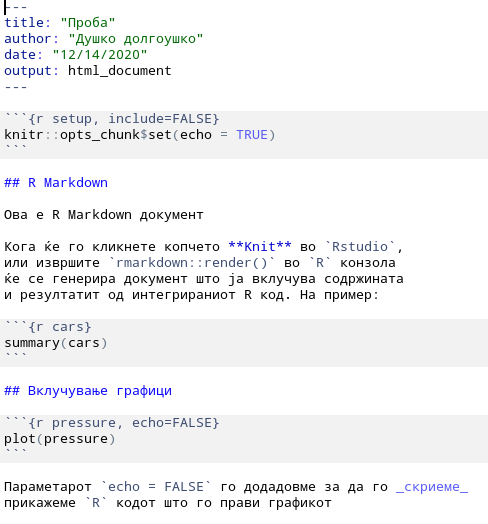
\includegraphics{www/rmd.png}
\caption{Пример за еден едноставен Rmd документ што прикажува текст, код, и резултати}
\end{figure}

Откако ќе го сплетеме овој документ, добиваме:

\begin{figure}
\centering
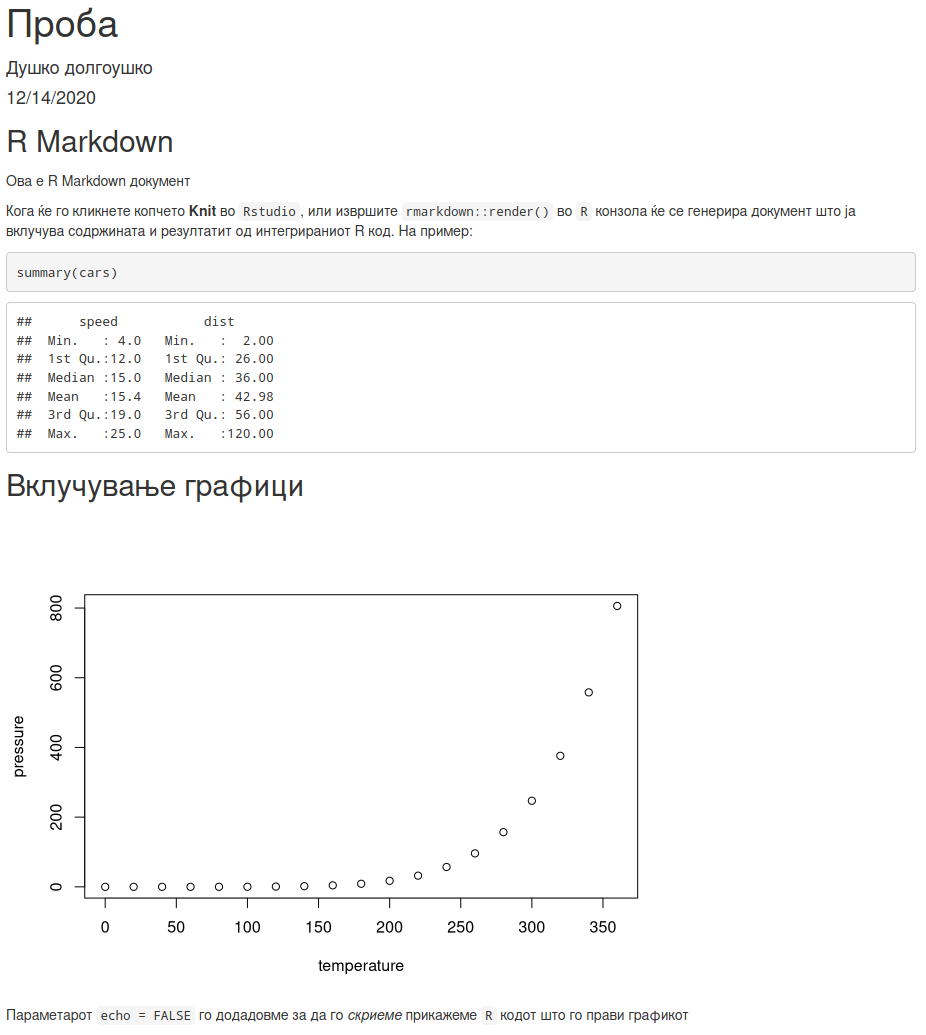
\includegraphics{www/rmd-rendered.png}
\caption{HTML документ креиран со плетењето на горниот Rmd код}
\end{figure}

Ова навистина само ја допира површината на тоа што е можно да се направи со алатките како \texttt{rmarkdown} и \texttt{knitr}. Имајќи во предвид дека крајните документи се \texttt{HTML}, \texttt{LaTex}, или \texttt{MS\ Word}, голем дел од богатсвото на можности на овие далеку поопширни \texttt{markup} системи ќе ви бидат достапни кога пишувате анализи во \texttt{Rmd}. Така да, ако сакате да вклучите лого од вашата организација, посебен фонт, специјално форматирње на маргини, пагинација, итн, сето тоа ќе можете тоа да го направите со стандардни медоти достапни во \texttt{HTML} или \texttt{LaTeX} (ЛИНКОВИ \citet{NOCI}??).

\hypertarget{ux438ux437ux432ux435ux448ux442ux430ux438-ux441ux43e-ux43fux430ux440ux430ux43cux435ux442ux440ux438}{%
\section{Извештаи со параметри}\label{ux438ux437ux432ux435ux448ux442ux430ux438-ux441ux43e-ux43fux430ux440ux430ux43cux435ux442ux440ux438}}

Она што за нас е посебно корисно и интересно, е користењето на оваа платформа за писмено програмирање за пишување на \href{https://rmarkdown.rstudio.com/developer_parameterized_reports.html\%23parameter_types\%2F}{параметризирани извештаи}. Што значи ова? Па доколку имате некоj стандарден сет на анализи кои треба да ги повторите за сите градови во Македонија, можете да го извршите вашиот \texttt{Rmd} извештај со параметар за тоа кој град треба да биде обработен. Во самиот изворен код на извештајот, дефинирате \texttt{yaml} преамбула налик на следната

\begin{verbatim}
---
title: Мој Извештај
output: html_document
params:
  grad: Tetovo
---
\end{verbatim}

Ова креира листа на параметри со името \texttt{params} која е достапна во \texttt{R} средината за време на извршувањето на документот, чијшто елементи може да ги употребите на следниот начин:

\begin{Shaded}
\begin{Highlighting}[]
\NormalTok{params}\OperatorTok{$}\NormalTok{grad}
\end{Highlighting}
\end{Shaded}

Доколку имаме некоја функција во нашиот извештај која се извршува пред правење на некој график за одреден град:

\begin{Shaded}
\begin{Highlighting}[]
\KeywordTok{library}\NormalTok{(dplyr)}
\NormalTok{filtriraj_gradovi <-}\StringTok{ }\ControlFlowTok{function}\NormalTok{(podatoci, potreben_grad) \{}
\NormalTok{  podatoci }\OperatorTok\StringTok{ }\NormalTok{dplyr}\OperatorTok{::}\KeywordTok{filter}\NormalTok{(grad }\OperatorTok{==}\StringTok{ }\NormalTok{potreben_grad)}
\NormalTok{\}}
\end{Highlighting}
\end{Shaded}

Тогаш можете параметарот даден во преамбулата да го искористите при повикувањето на фунцкијата, и сите натамошни резултати ќе бидат посветени на градот што сме го пратиле како параметар:

\begin{Shaded}
\begin{Highlighting}[]
\CommentTok{# претходен код и текст}
\KeywordTok{filtriraj_gradovi}\NormalTok{(}\DataTypeTok{podatoci =}\NormalTok{ moi_podatoci, }\DataTypeTok{potreben_grad =}\NormalTok{ params}\OperatorTok{$}\NormalTok{grad)}
\CommentTok{# натамошен код и текст}
\end{Highlighting}
\end{Shaded}

За да ги направиме сите извештаи поврзо, во можеме да го повикуваме извршувањето во \texttt{R} конзола:

\begin{Shaded}
\begin{Highlighting}[]
\NormalTok{rmarkdown}\OperatorTok{::}\KeywordTok{render}\NormalTok{(}\DataTypeTok{input =} \StringTok{"mojizvestaj.Rmd"}\NormalTok{, }\DataTypeTok{params =} \KeywordTok{list}\NormalTok{(}\StringTok{"Tetovo"}\NormalTok{))}
\end{Highlighting}
\end{Shaded}

Оттука, во \texttt{R} можеме дури и да напишеме \texttt{for} циклус со кој што ќе ги процесираме сите градови наеднаш и ќе генерираме посебен \texttt{HTML}, \texttt{PDF} или \texttt{MS\ Word} документ се секој град:

\begin{Shaded}
\begin{Highlighting}[]
\NormalTok{gradovi <-}\StringTok{ }\KeywordTok{c}\NormalTok{(}\StringTok{"Tetovo"}\NormalTok{, }\StringTok{"Gostivar"}\NormalTok{, }\StringTok{"Debar"}\NormalTok{, }\StringTok{"Berovo"}\NormalTok{, }\StringTok{"Dojran"}\NormalTok{) }\CommentTok{# ...}
\ControlFlowTok{for}\NormalTok{ ( i }\ControlFlowTok{in}\NormalTok{ gradovi) \{}
  \KeywordTok{message}\NormalTok{(}\StringTok{"Подготвувам извештај за: "}\NormalTok{, i)}
\NormalTok{  rmarkdown}\OperatorTok{::}\KeywordTok{render}\NormalTok{(}\DataTypeTok{input =} \StringTok{"pateka/do/mojizvestaj.Rmd"}\NormalTok{, }\DataTypeTok{params =} \KeywordTok{list}\NormalTok{(i))}
\NormalTok{\}}
\end{Highlighting}
\end{Shaded}

Како оваа стратегија ја подобрува повторливоста на нашите анализи? Доколку немаме извештаи со параметри можеме да замислиме две стратегии. Првата, имаме еден главен \texttt{izvestaj.Rmd} којшто никогаш не го менуваме и правиме копии за секој град, така што набрзо нашата работна средина станува невозможна за менаџирање на долг рок:

\begin{verbatim}
izvestaj.Rmd
tetovo-izvestaj.Rmd
debar-izvestaj.Rmd
skopje-izvestaj.Rmd
skopje-izvestaj-juni.Rmd
skopje-izvestaj-juni-specijalen-so-logo.Rmd
kichevo-izvestaj-avgust-2019.Rmd
kicevo-izvestaj-avgust.Rmd
\end{verbatim}

Втората, имаме еден \texttt{izvestaj.Rmd} којшто го менуваме директно и секогаш мора да го отвориме, промениме, и извршиме рачно. Така да кога ќе стигнат новите податоци следниот месец имаме 2-3 часа работа да го промениме градот во функцијата горе триесетина пати.

Дури и да го имате потребното време за вакви активности, очигледно е дека со овие опции е далеку полесно да направите грешка отколку со извештајот со параметри, којшто го пишувате еднаш и можете да го користите секогаш кога ќе ви треба без да го менувате изворниот код. Доколку треба да се измени или подобри извештајот, тоа се прави со промена на само еден документ, не треба да се сетите дека \texttt{kopje-izvestaj-juni-specijalen-so-logo.Rmd} треба да се промени засебно бидејќи има нешто специфично.

\hypertarget{ux441ux43bux435ux434ux43dux438-ux447ux435ux43aux43eux440ux438}{%
\section{Следни чекори}\label{ux441ux43bux435ux434ux43dux438-ux447ux435ux43aux43eux440ux438}}

Околината на \texttt{rmarkdown} и \texttt{knitr} е особено богата со алатки за посебни намени што навистина можат да придонесат кон поголема транспарентност, повторливост на вашите анализи и генерално кон поголема продуктивност во вашата работа. Подолу наведуваме само неколку од овие алатки:

\begin{itemize}
\tightlist
\item
  креирање презентации (на пример: тука, тука, тука)
\item
  креирање \emph{интерактивни} \texttt{Rmd} документи што користат \texttt{Shiny\ server} позадина (линк)
\item
  креирање стилизирани HTML документи со prettyprint (линк)
\item
  креирање на книги со bookdown (како овој текст)
\item
  креирање на едноставни \texttt{Rmarkdown} вебсајти со \texttt{rmarkdown::render\_site} (\url{https://rmarkdown.rstudio.com/lesson-13.html})
\item
  креирање на дашбоарди со \texttt{flexdashboard}
\end{itemize}

\hypertarget{ux43fux43eux432ux442ux43eux440ux43bux438ux432ux438-ux43fux440ux43eux435ux43aux442ux438}{%
\chapter{Повторливи проекти}\label{ux43fux43eux432ux442ux43eux440ux43bux438ux432ux438-ux43fux440ux43eux435ux43aux442ux438}}

Во претходните две поглавја разгледавме како можеме нашиот едноставен код да го конвертираме во скрипта која ќе биде лесна за користење и до некоја мера издржлива во различни работни средини (РЕФ 4) и како да составиме повторлив извештај со повеќе табели и графици со помош на \texttt{Rmd} (REF 5). Но како што напоменавме, сеуште правиме некои претпоставки за начинот на кој ќе биде користена скриптата и за ресурсите кои ќе им бидат достапни на корисниците. Една од овие претпоставки беше дека колегите кои ќе ја користат нашата скрипта ќе имаат адекватни табели за обработување. Ова е до некоја мера разумна претпоставка доколку скриптата се користи рамките на една организација, или доколку типот на табели кои ги обработува се доволно познати и распространети. Но ваквите случаи, иако значајни, претставуваат само дел инстанците кога треба да разговараме за повторливи анализи. Да разгледаме некои примери:

Пример 1: Работите во невладина организација чијшто фунцкионирање зависи од надворешни грантови, како од македонски така и од странски извори. Се почесто, донорите поставуаат услови за активностите кои тие ги подджуваат, дека сите податоци кои вашата организација ги собира (преку анкети, истражувања, и контакти) како и сите анализи на тие податоци треба да се транспарентни и повторливи (РЕФ ????: Нели има некоја ЕУ регулатива за ова). Што во пракса значи дека со завршниот извештај за проектот во кој ги презентирате резултатите, вие ќе треба исто така да покажете јавна депозиција на податоците и изворниот код користен да се добиат презентираните резултати. Со други зборови, пред вас е задача за повторлива анализа, слично на она што го видовме погоре, но со далеку повеќе код, скрипти, и податоци. Критичната разлика е во контекстот. Ако претходно претпоставуваме дека корисниците на нашиот повторлив код ќе имаат пристап до податоците, сега кога треба да ги споделиме податоците \emph{надвор} од нашата организација, таа претпоставка веќе не важи. Значи ни треба начин да го споделиме нашиот програмски код заедно со податоците кои ги обработуваме, инаку никој надвор од нашата организација нема да може да ја повтори анализата.

Пример 2: Работите во индустриска лабораторија каде што вашата работа е да правите статистичка обработка на експериментални резултати или анализи за контрола на квалитет. Вашата организација повторно фунцкионира преку надворешни грантови или клиенти кои очекуваат дека резултатите од вашата лабораторија ќе може да бида независно потврдени. Во пракса ова повторно значи објавување на повторлив проект, со податоци и програмски код, кој што ќе работи во контекст многу различен од вашата лабораторија.

Пример 3: Накратко, бидејќи патернот е јасен. Вие сте научен истражувач на некој универзитет или институт. Вашата работа зависи од објавување трудови и аплицирање за грантови. Се поголем број на научни журнали имаат стриктни барања за транспарентни и повторливи анализи без кои нема ни да го рецензираат трудот. Вас ви треба повторлив проект.

Во ова поглавје ќе се запознаеме со две стратегии за организирање на повторливи проекти. Првата стратегија (Направи сам) е едноставна за поставување и не зависи од дополнителна инфраструктура (додатни библиотеки), но ако проектот е комплексен, оваа опција може да бара повеќе грижа, особено за стабилност на подолг рок. Втората стратегија е да се повикаме на некоја веќе готова платформа за поставување на безбедна структура за повторливи проекти. Втората стратегија генерално треба да се преферира, но имајќи во предвид дека секој нов пакет си бара одреден период на запознавање и дека во некои случаи првата опција е сосема адекватна, ќе збориваме за двете стратегии.

\hypertarget{ux441ux442ux440ux430ux442ux435ux433ux438ux458ux430-1-ux43dux430ux43fux440ux430ux432ux438-ux441ux430ux43c}{%
\section{Стратегија 1: Направи сам}\label{ux441ux442ux440ux430ux442ux435ux433ux438ux458ux430-1-ux43dux430ux43fux440ux430ux432ux438-ux441ux430ux43c}}

\hypertarget{ux441ux442ux440ux443ux43aux442ux443ux440ux430}{%
\subsection{Структура}\label{ux441ux442ux440ux443ux43aux442ux443ux440ux430}}

Креирање безбедна структура за повторливост во основа е едноставно. Да речеме дека имаме извештај со два графикони и три табели, и дека секој график и табела се базирани на различни сетови на податоци. Имајќи ги во предвид нашите цели:

\begin{itemize}
\tightlist
\item
  да направиме што е можно помалку претпоставки за средината во којашто ќе биде повторена нашата анализа и\\
\item
  да направиме што е можно полесно да се снајде некој без никакво претходно искуство со нашиот проект
\end{itemize}

можеме секој елемент од нашиот извештај да го енкапсулираме во посебен фолдер. Во секој фолдер мора да ги вклучиме \textbf{податоците и програмскиот код} коишто се неопходни за ре-креирање на графиконот или табелата. За детални објаснувања, можеме во (фали нешто тука?) да вклучиме \texttt{README} фалј во оние фолдери каде што е неопходно. Главен \texttt{README} фалј на првото ниво на нашиот проект \textbf{мора да биде вклучен}. Тука, го опишуваме нашиот проект, што подетално тоа подобро, и даваме објаснување за како да се користат податоците и кодот којшто е вклучен во субфолдерите. Ова е особено важно доколку скриптите зависат една од друга и треба да се извршат во некој редослед, на пример ако мора прво да го извршиме кодот во \texttt{tabela\_1} пред да можеме да работиме со \texttt{tabela\_2}.

Во нашиот случај, со два графикони и три табели сите со различни податоци, би ја имаме следната структура:

\begin{verbatim}
strategija_1/
├── grafik_1
│   ├── code_grafik_1.R
│   └── data_grafik_1.csv
├── grafik_2
│   ├── code_grafik_2.R
│   └── data_grafik_2.csv
├── README
├── tabela_1
│   ├── code_tabela_1.R
│   └── data_tabela_1.csv
├── tabela_2
│   ├── code_tabela_2.R
│   └── data_tabela_2.csv
└── tabela_3
    ├── code_tabela_3.R
    └── data_tabela_3.csv
\end{verbatim}

Доколку графиконите 1 и 2 се базирани на исти податоци како табелите 1 и 2, тогаш можеме да ги групираме, со што би избегнало непотребно копирање на истите податоци на две места:

\begin{verbatim}
strategija_1/
├── grafik_1
│   ├── code_grafik_1.R
│   ├── code_tabela_1.R
│   └── data_grafik_1.csv
├── grafik_2
│   ├── code_grafik_2.R
│   ├── code_tabela_2.R
│   └── data_grafik_2.csv
├── README
└── tabela_3
    ├── code_tabela_3.R
    └── data_tabela_3.csv
\end{verbatim}

Но генерално, при одлучување за структурата на проектот треба да си го поставиме прашањето „како најлесно ќе се снајде некој што никогаш претходно нема работено со овие податоци или тип на анализи?{}``. Доколку одговорот на ова прашање сугерира да се копираат истите податоци на две места, и податоците се доволно мали да го дозволат тоа, тогаш е подобро да се направи вишокот отколку да се направи ре-анализата покомплицирана.

\hypertarget{ux43fux440ux435ux434ux43dux43eux441ux442ux438}{%
\subsection{Предности}\label{ux43fux440ux435ux434ux43dux43eux441ux442ux438}}

Како оваа стратегија овозможува повторливост? Доколку нашиот код ги следи принципите за кои збориваме претходно, спарувањето на податоците со кодот што треба да се користи за нивна обработка во еден фолдер изолирани од остатокот на проектот значи дека:

\begin{itemize}
\tightlist
\item
  шансите корисникот на нашиот проект да ги помеша фајловите се минимални,\\
\item
  нашиот код може да биде поедноставен бидејќи вчитува податоци во истиот фолдер, и конечно
\item
  сите резултати од извршувањето на нашиот код (на пример пдф од графикон) ќе се зачуваат во истиот фолдер.
\end{itemize}

Оваа едноставна, линеарна поврзаност е веројатно најбезбедна од аспект на поставување и користење подоцна од некој кој нема никакво претходно познавање. Дополнително, ваквата структура овозможува модуларност, во смисла на тоа дека секоја табела или графикон може да се ре-креира независно од остатокот на анализата, ако, на пример, нашиот соработник или рецензент сака да провери само одреден аспект на истражувањето.

\hypertarget{ux43dux435ux434ux43eux441ux442ux430ux442ux43eux446ux438}{%
\subsection{Недостатоци}\label{ux43dux435ux434ux43eux441ux442ux430ux442ux43eux446ux438}}

Главните недостатоци на оваа стратегија се непотребното повторување на код или податоци (не секогаш, но често), и тоа што оваа организација станува незгодна ако имаме голем или комплициран извештај со многу анализи коишто би сакале да ги одделиме.

Можното непотребно повторување да податоци веќе спомнавме погоре како разлика помеѓу недостатоците на дуплицирање наспроти предноста што копирањето на една табела на две места може да подобри леснотијата на користење. Имено, доколку некоја скрипта има соодветно именувана табела што ја користи во соодветно именуван фолдер, тогаш дури и истата табела да се јави под друго име во друг фолдер каде што се отвара од друга скрипта, тоа не создава забуна. Од друга страна, доколку истата табела, под исто име, се наоѓа во заедничи фолдер \texttt{Табели}, тогаш треба за двете скрипти да објасниме дека ја користат истата табела и двете скрипти треба да повикуваат табела што е сместена надвор од соодветните фолдери. Второто сценарио е малку покомплицирано, и доколку табелата во прашање е доволно мала (во смисол на меморија) тогаш од перспектива на корисник кој прв пат го гледа проектот можеби не е проблем доколку се јавува два пати.

Сепак, генералната препорака е дека најдобро е да се избегне дупликација на податоци, бидејќи податоците се (типично) најголемиот (во смисол на меморија) дел од нашиот пакет, а сакаме нашиот пакет да биде што попортабилен.

За повторувањето на програмски код имаме слична дилема. Доколку нашите табели или графици, кои ги правиме со посебни скрипти во посебни фолдери, имаат делови со идентичен код (на пример сите скрипти ги прават истите проверки за табелите, или сите скрипти за табела ја прават истата сумација по групи), тогаш можеме делот од кодот што се повторува да го изолираме во посебна скрипта што сите други скрипти ќе ја повикуваат. Оваа опција е подобра бидејќи доколку најдеме грешка или сакаме да направиме некое подобрување, тоа го правиме само во скриптата со заеднички код, додека пак доколку тој код се дуплицира во повеќе скрипти, ќе треба да ги промениме сите. Во ваков случај со изолиран заеднички код, нашата структура може да се промени во нешто налик на следниот дијаграм.

\begin{verbatim}
strategija_1/
├── README
├── zaednicki-kod.R
├── grafik_1
│   ├── code_grafik_1.R
│   ├── code_tabela_1.R
│   └── data_grafik_1.csv
├── grafik_2
│   ├── code_grafik_2.R
│   ├── code_tabela_2.R
│   └── data_grafik_2.csv
└── tabela_3
    ├── code_tabela_3.R
    └── data_tabela_3.csv
\end{verbatim}

Вториот недостаток, незгодноста кога проектот станува голем и комплициран, станува јасен со претходниот дијаграм. Кога скриптите, и фунцкии внатре во скриптите, почнуваат да стануваат зависни една од друга, предностите на линерано изолирање на кодот и податоците почнуваат да се смалуваат. На пример, ако \texttt{code\_tabela\_3.R} има функција \texttt{sumiraj-po-grupi()} која повикува две функции од \texttt{zaednicki-kod.R} и ја вчитува табелата што резултира од модулот \texttt{grafik\_2}, тогаш немаме баш линеарна зависност туку нешто покомплицирано. И иако сеуште можеме рачно да ги организираме ваквите врски помеѓу код и податоци, веројатно е време да разгледаме други опции за организирање на нашиот проект.

\hypertarget{ux441ux442ux440ux430ux442ux435ux433ux438ux458ux430-2-ux444ux43eux440ux43cux430ux43bux435ux43d-r-ux43fux430ux43aux435ux442-ux438ux43bux438-ux43dux435ux43aux43eux458ux430-ux43fux43eux435ux434ux43dux43eux441ux442ux430ux432ux435ux43dux430-ux432ux430ux440ux438ux458ux430ux43dux442ux430}{%
\section{\texorpdfstring{Стратегија 2: Формален \texttt{R} пакет или некоја поедноставена варијанта}{Стратегија 2: Формален R пакет или некоја поедноставена варијанта}}\label{ux441ux442ux440ux430ux442ux435ux433ux438ux458ux430-2-ux444ux43eux440ux43cux430ux43bux435ux43d-r-ux43fux430ux43aux435ux442-ux438ux43bux438-ux43dux435ux43aux43eux458ux430-ux43fux43eux435ux434ux43dux43eux441ux442ux430ux432ux435ux43dux430-ux432ux430ux440ux438ux458ux430ux43dux442ux430}}

\hypertarget{ux441ux442ux440ux443ux43aux442ux443ux440ux430-1}{%
\subsection{Структура}\label{ux441ux442ux440ux443ux43aux442ux443ux440ux430-1}}

Разгледувајќи ја првата стратегија за организирање на повторливи проекти дојдовме до моментот кога зависностите помеѓу нашиот код и податоци почнуваа да стануваат не-линеарни. Од една страна, неколку скрипти можат да ги користат истите податоци и да повикуваат функции од една скрипта за заеднички код, од друга страна, една скрипта може да зависи од резултатите на повеќе други прекурсори. Кога нашиот проект ќе ја стигне оваа фаза, тогаш подобро е да ја напуштиме линеарната структура што изолира еден сет на податоците и нивната обработка од остатокот на пакетот и да го реорганизираме проектот така што податоците, кодот, извештате, итн, ќе бидат во засебни фолдери. Во овој случај, структурата на проектот може да биде нешто налик на следниот дијаграм:

\begin{verbatim}
strategija_2/
├── izvestai
├── podatoci
├── README
└── skripti
\end{verbatim}

Доколку некогаш сте ја погледнале структурата на еден формален \texttt{R} пакет (под „формален„ мислиме пакет или библиотека која што може да се инсталира и повика со \texttt{library(mojpaket)}), веднаш ќе ги забележите сличностите:

\begin{figure}
\centering
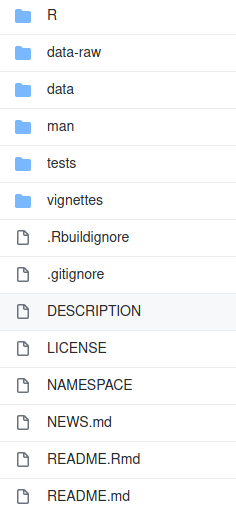
\includegraphics{www/package-structure.png}
\caption{Структура на еден формален \texttt{R} пакет (библиотека)}
\end{figure}

Сиот програмски код е изолиран во посебен фолдер (\texttt{skripti} или \texttt{R}), податоците се во фолдери посветени на податоци (\texttt{podatoci} или \texttt{data} или \texttt{data-raw}), главниот директориум во двата случаи има \texttt{README} фајл кој ја објаснува намената на пакетот и укажува како може да се користат спакувануте компоненти, итн.

Како работиме во оваа средина? Без разлика колку скрипти имаме, со колку функции во нив, и колку комплексни се зависностите помеѓу нив:

\begin{enumerate}
\def\labelenumi{\arabic{enumi}.}
\tightlist
\item
  сите тие скрипти ги вчитуваме во нашата \texttt{R} средина (global environment, \texttt{.GlobalEnv}), така што кога една фунција повикува втора функција не мора да се сетиме во која скрипта живее таа функција\\
\item
  сите тие скрипти вчитуваат податоци кои се наоѓаат во \texttt{podatoci} и никаде на друго место\\
\item
  сите тие скрипти зачувуваат продукти (табели, графици, HTML/PDF извештаи) во \texttt{izvestai}
\end{enumerate}

На ваков начин, ја елиминараме потрабата од копирање на податоци или код, и секоја компонента, дали е тоа изворен код или податоци, се јавува само еднаш во нашиот пакет.

\hypertarget{ux43fux43eux441ux442ux430ux432ux443ux432ux430ux45aux435}{%
\subsection{Поставување}\label{ux43fux43eux441ux442ux430ux432ux443ux432ux430ux45aux435}}

Поставувањето на ваков повторлив проект може повторно да оди рачно, едноставно правиме фолдери за податоци, изборен код, итн. Но исто таке можеме да искористиме постоечки функции и пакети кои го прават овој чекор полесен. Иако има многу решенија достапни решенија, ќе тука ќе споменеме две опции. Прво, можеме да ја искористиме функционалноста за креирање формални \texttt{R} пакети, дури немаме намера да го објавуваме нашиот пакет. Кодот е едноставен:

\begin{Shaded}
\begin{Highlighting}[]
\KeywordTok{library}\NormalTok{(devtools)}
\KeywordTok{library}\NormalTok{(usethis)}
\NormalTok{devtoos}\OperatorTok{::}\KeywordTok{create}\NormalTok{(}\DataTypeTok{path =} \StringTok{"mojpaket"}\NormalTok{)}

\NormalTok{podatoci1 <-}\StringTok{ }\KeywordTok{read.csv}\NormalTok{(}\StringTok{"~/Desktop/moi-podatoci.csv"}\NormalTok{)}
\NormalTok{usethis}\OperatorTok{::}\KeywordTok{use_data}\NormalTok{(}\StringTok{"podatoci1"}\NormalTok{)}
\end{Highlighting}
\end{Shaded}

Извршувањето на горните линии ќе креира структура налик на следната:

\begin{verbatim}
mojpaket/
├── DESCRIPTION
├── NAMESPACE
├── data
└── R
\end{verbatim}

Понатаму, како додавате документација, вињети, или тестови, можете да генерирате соодветни фолдери полу-автоматски. За далеку повеќе детали околу овие процедури, ве повикуваме да ја погледнете книгата за \texttt{R} пакети од Хадли Викам (\citep{wickham2015r}).

Втората опција за креирање на ваква структура за повторлив проект е преку користење на пакети посветени кон токму тоа: да олеснат повторливи анализи/истражувања/извештаи преку автоматизирање на некој од компонентите на повторливост кои ги дискутиравме до сега. Има повеќе вакви пакети: \texttt{prodigenr}, \texttt{makeProject}, \texttt{ProjectTemplate}, \texttt{fertile}, \texttt{goodpractice}, итн кои специјализираат кон различни аспекти (дали структура на проектот, проверки на кодот, итн). Овде, накратко, ќе се запознаеме со основната функционалност на пакетот \texttt{prodigenr} кој овозможува креирање на структура налик на формален \texttt{R} пакет но без (понекогаш непотребниот) багаж кој доаѓа со развивањето и користењето на еден формален \texttt{R} пакет.

\begin{Shaded}
\begin{Highlighting}[]
\KeywordTok{library}\NormalTok{(prodigenr)}
\KeywordTok{setup_project}\NormalTok{(}\StringTok{"data/mojproekt2"}\NormalTok{)}
\end{Highlighting}
\end{Shaded}

Потоа, доколку го погледнеме направениот проект ја имаме следната структура:

\begin{verbatim}
mojproekt2/
├── data
│   └── README.md
├── DESCRIPTION
├── doc
│   └── README.md
├── mojproekt2.Rproj
├── R
│   ├── fetch_data.R
│   ├── README.md
│   └── setup.R
├── README.md
└── TODO.md
\end{verbatim}

На пример, скриптата \texttt{setup.R} доаѓа со објаснување како да ги организираме нашите скрипти/функции со цел да бидат достапни за време на интерактивната сесија. Додека пак скриптата \texttt{fetch\_data.R} не насочува кон тоа како да ги собираме и подготвиме табелите со податоци за зачувување во \texttt{data/} и понатамошно користење. Како и во еден формален пакет, фајлот \texttt{DESCRIPTION} дава инструкции за зависностите на нашиот код (не-стандардни \texttt{R} пакети). Како и секогаш, ве покануваме да ја прочитате документацијата на пакетот (на пример \texttt{library(help="prodigenr")}) за повеќе детали.

\hypertarget{ux43fux440ux435ux434ux43dux43eux441ux442ux438-1}{%
\subsection{Предности}\label{ux43fux440ux435ux434ux43dux43eux441ux442ux438-1}}

Очигледно има добри причини зошто би сакале нашиот повторлив проект да има структура слична на формален \texttt{R} пакет. Еден \texttt{R} пакет може да се инсталира и користи без проблем на било кој компјутер, има ефективна документација со вградени упатства за употреба и подолги вињети за специјални случаи, има екплицитно менаџирање на зависностите, и единични тестови (unit tests) кои што проверуваат дали секоја фунцкија го дава очекуваниот резултат во различни контексти.

\hypertarget{ux43dux435ux434ux43eux441ux442ux430ux442ux43eux446ux438-1}{%
\subsection{Недостатоци}\label{ux43dux435ux434ux43eux441ux442ux430ux442ux43eux446ux438-1}}

Може да се најдат недостатоци во било кој систем, и секако оваа структура може сеуште да се подобрува, но за робустна организација на вашите повторливи проекти веројатно треба да се држите до некоја од алтернативите дискутирани тука. Она што може да се спомене, не како недостаток, туку предупредување, е дека навинкувањето и целосно искористување на ова структура ќе бара малку повеќе време и учење, како за оној кој го подготвува проектот така и за корисниците.

\hypertarget{ux43aux43eux43dux442ux440ux43eux43bux430-ux43dux430-ux438ux437ux432ux43eux440ux43dux438ux43eux442-ux43aux43eux434-git-github}{%
\chapter{Контрола на изворниот код (git / GitHub)}\label{ux43aux43eux43dux442ux440ux43eux43bux430-ux43dux430-ux438ux437ux432ux43eux440ux43dux438ux43eux442-ux43aux43eux434-git-github}}

Контрола на изворниот код (или дури и на целата содржина во еден истражувачки проект) е можна со помош на користење на алатки како \texttt{Git}. Употребата на \texttt{Git} е олесната благодарение на веб страниците како што се \texttt{Github} или \texttt{Gitlab}.

Контролата на содржината е корисна. Кога пишувате текст или код и потоа менувате, \texttt{Git} овозможува да ги видите тие промени, да споредите, или да ги вратите назад. Може да се каже дека тој е многу напредна верзија на вообичаното \texttt{track\ changes} што се користи во алатки како \texttt{MS\ Word}.

Сепак, детален осврт на можностите и особеносите на \texttt{Git} не е тема овде. За тие што се заинтересирани и сакаат да истражуваат постојат ресурси кои детално ги објаснуваат сите детали. На пр. \url{https://git-scm.com/book/en/v2}

Овде ќе се осврнеме само на една можност која што ја нуди \texttt{Github} за презентирање на HMTL.

\hypertarget{not-too-much-about-git-of-course-that-is-not-the-point-anyway}{%
\chapter{not too much about git (of course that is not the point anyway)}\label{not-too-much-about-git-of-course-that-is-not-the-point-anyway}}

\hypertarget{just-about-creating-a-github-repo-where-you-can-push-rmd-in-main-and-html-in-gh-pages-thus-making-your-reserarch-public-on-the-web-mostly-working-thourgh-r-studio-exept-for-creating-the-account-on-gh.}{%
\chapter{just about creating a github repo where you can push rmd in main and html in gh-pages thus making your reserarch public on the web mostly working thourgh r studio exept for creating the account on gh.}\label{just-about-creating-a-github-repo-where-you-can-push-rmd-in-main-and-html-in-gh-pages-thus-making-your-reserarch-public-on-the-web-mostly-working-thourgh-r-studio-exept-for-creating-the-account-on-gh.}}

\hypertarget{ux440ux435ux444ux435ux440ux435ux43dux446ux438-httpsgit-scm.combookenv2}{%
\subsection{\texorpdfstring{референци: \url{https://git-scm.com/book/en/v2}}{референци: https://git-scm.com/book/en/v2}}\label{ux440ux435ux444ux435ux440ux435ux43dux446ux438-httpsgit-scm.combookenv2}}

  \bibliography{book.bib,packages.bib,pckg.bib}

\end{document}
